% $Id: template.tex 11 2007-04-03 22:25:53Z jpeltier $

% \documentclass[anonymous=True]{vgtc}             % final (conference style)
% \documentclass[review]{vgtc}         % review
%\documentclass[widereview]{vgtc}       % wide-spaced review
\documentclass[preprint]{vgtc}        % preprint
%\documentclass[electronic]{vgtc}       % electronic version

%% Uncomment one of the lines above depending on where your paper is
%% in the conference process. ``review'' and ``widereview'' are for review
%% submission, ``preprint'' is for pre-publication, and the final version
%% doesn't use a specific qualifier. Further, ``electronic'' includes
%% hyperreferences for more convenient online viewing.

%% Please use one of the ``review'' options in combination with the
%% assigned online id (see below) ONLY if your paper uses a double blind
%% review process. Some conferences, like IEEE Vis and InfoVis, have NOT
%% in the past.

%% Figures should be in CMYK or Grey scale format, otherwise, colour 
%% shifting may occur during the printing process.

%% These few lines make a distinction between latex and pdflatex calls and they
%% bring in essential packages for graphics and font handling.https://v2.overleaf.com/project/5b75b33a3afa9339f3dd2a2d
%% Note that due to the \DeclareGraphicsExtensions{} call it is no longer necessary
%% to provide the the path and extension of a graphics file:
%% \includegraphics{diamondrule} is completely sufficient.
%%
\ifpdf%                % if we use pdflatex
 \pdfoutput=1\relax          % create PDFs from pdfLaTeX
 \pdfcompresslevel=9         % PDF Compression
 \pdfoptionpdfminorversion=7     % create PDF 1.7
 \ExecuteOptions{pdftex}
 \usepackage{graphicx}        % allow us to embed graphics files
 \DeclareGraphicsExtensions{.pdf,.png,.jpg,.jpeg} % for pdflatex we expect .pdf, .png, or .jpg files
\else%                 % else we use pure latex
 \ExecuteOptions{dvips}
 \usepackage{graphicx}        % allow us to embed graphics files
 \DeclareGraphicsExtensions{.eps}   % for pure latex we expect eps files
\fi%

% coloring author
\usepackage[usenames,dvipsnames,svgnames,table]{xcolor}
\newcommand{\todo}[1]{{}}
\newcommand{\note}[1]{{}}
\newcommand{\skyerevise}[1]{{\color{blue} #1}}
\newcommand{\gregoriorevise}[1]{{\color{cyan} #1}}
\newcommand{\haleyrevise}[1]{{\color{orange}#1}}
\newcommand{\wenborevise}[1]{{\color{green} #1}}
\newcommand{\yihsunrevise}[1]{{\color{lightgray} #1}}
\newcommand{\tristanrevise}[1]{{\color{red}{#1}}} 

\newcommand{\skye}[1]{{ #1}}
\newcommand{\gregorio}[1]{{ #1}}
\newcommand{\haley}[1]{{#1}}
\newcommand{\wenbo}[1]{{ #1}}
\newcommand{\yihsun}[1]{{ #1}}
\newcommand{\tristan}[1]{{{#1}}} 

%% it is recomended to use ``\autoref{sec:bla}'' instead of ``Fig.~\ref{sec:bla}''
\graphicspath{{figures/}{pictures/}{images/}{./}} % where to search for the images

\usepackage{microtype}         % use micro-typography (slightly more compact, better to read)
\PassOptionsToPackage{warn}{textcomp} % to address font issues with \textrightarrow
\usepackage{textcomp}         % use better special symbols
\usepackage{mathptmx}         % use matching math font
\usepackage{times}           % we use Times as the main font
\renewcommand*\ttdefault{txtt}     % a nicer typewriter font
\usepackage{cite}           % needed to automatically sort the references
\usepackage{tabu}           % only used for the table example
\usepackage{booktabs}         % only used for the table example
%% We encourage the use of mathptmx for consistent usage of times font
%% throughout the proceedings. However, if you encounter conflicts
%% with other math-related packages, you may want to disable it.


%% If you are submitting a paper to a conference for review with a double
%% blind reviewing process, please replace the value ``0'' below with your
%% OnlineID. Otherwise, you may safely leave it at ``0''.
\onlineid{0}

%% declare the category of your paper, only shown in review mode
\vgtccategory{Research}

%% allow for this line if you want the electronic option to work properly
\vgtcinsertpkg

%% In preprint mode you may define your own headline.
%\preprinttext{To appear in an IEEE VGTC sponsored conference.}

%% Paper title.

\title{HyperTuner: Visual Analytics for Hyperparameter Tuning by Professionals}

%% This is how authors are specified in the conference style

%% Author and Affiliation (single author).
%%\author{Roy G. Biv\thanks{e-mail: roy.g.biv@aol.com}}
%%\affiliation{\scriptsize Allied Widgets Research}

%% Author and Affiliation (multiple authors with single affiliations).
%%\author{Roy G. Biv\thanks{e-mail: roy.g.biv@aol.com} %
%%\and Ed Grimley\thanks{e-mail:ed.grimley@aol.com} %
%%\and Martha Stewart\thanks{e-mail:martha.stewart@marthastewart.com}}
%%\affiliation{\scriptsize Martha Stewart Enterprises \\ Microsoft Research}

% Author and Affiliation (multiple authors with single affiliations).
\author{Tianyi Li\thanks{e-mail:tianyi.li@cloudera.com} 
\and Gregorio Convertino\thanks{e-mail:gconvertino@cloudera.com} 
\and Wenbo Wang \thanks{e-mail:wenbo@cloudera.com} 
\and Haley Most \thanks{e-mail:haley@cloudera.com} 
\and Tristan Zajonc \thanks{e-mail:tristanz@cloudera.com} 
\and Yi-Hsun Tsai \thanks{e-mail:yihsuntsai@cloudera.com}} 
\affiliation{\scriptsize UX Design and Cloudera Data Science Workbench \\ Cloudera }


%% Author and Affiliation (multiple authors with multiple affiliations)
% \author{Roy G. Biv\thanks{e-mail: roy.g.biv@aol.com}\\ %
%     \scriptsize Starbucks Research %
% \and Ed Grimley\thanks{e-mail: ed.grimley@aol.com}\\ %
%   \scriptsize Grimley Widgets, Inc. %
% \and Martha Stewart\thanks{e-mail: martha.stewart@marthastewart.com}\\ %
%   \parbox{1.4in}{\scriptsize \centering Martha Stewart Enterprises \\ Microsoft Research}}

%% Author and Affiliation (multiple authors with multiple affiliations)
% \author{UX Design Team\thanks{e-mail: @cloudera.com}\\ %
%     \scriptsize Cloudera %
% \and CDSW team\thanks{e-mail: @cloudera.com}\\ %
%   \scriptsize Cloudera % }
%% A teaser figure can be included as follows, but is not recommended since
%% the space is now taken up by a full width abstract.
%\teaser{
% 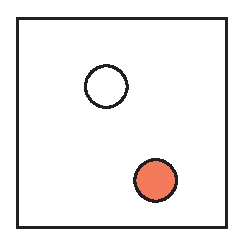
\includegraphics[width=1.5in]{sample.eps}
% \caption{Lookit! Lookit!}
%}

%% Abstract section.
\abstract{

While training a machine learning model, data scientists often need to determine a set of hyperparameters that configures structure and other characteristics of the model. The choice of hyperparameters can significantly influence the model performance, but determining good values can be a nuisance.
This paper reports on user needs for hyperparameter tuning and proposes a prototype to provide model-agnostic support for this process. 
We characterize the hyperparameter tuning process based on interviews with data science practitioners in industry. We identify opportunities to help the user gain insight into the role of hyperparameters on model performance and convergence, and tune hyperparameters through an iterative process guided by visual analytics. We present a prototype that implements our proposed design, which treats models as black boxes with hyperparameters and data as inputs and predictions and performance metrics as outputs. The feedback we collected from the same group of data science practitioners shows that the design leverages appropriate visual analytics to support the key steps of the hyperparameter tuning process, and also triggers further discussions on more advanced requirements such as automated tuning and debugging support. 

% %(1)Describing what was done. OLD VERSION
% When training machine learning models, data scientists often times need to determine a set of model parameters before the learning process begins. By contrast, the values of other parameters are learned via training. This paper focuses on designing model-agnostic support for tuning the \textit{model parameters} and, thus, optimize model performance. We analyze and characterize the status quo of the model tuning process through interviews with data science practitioners in industry. 
% %(2) Describing what was found (key results). Be specific about your key findings. Instead of “many” say “84%”.
% Treating models as black boxes with model parameters as inputs and derived performance metrics as outputs, we formulate a model parameter tuning workflow within a model tuning pipeline. In this context, we investigate how to provide appropriate visual assistance that can help data scientists find the sweet-spot setting for model parameters. We propose and evaluate a preliminary design that implements the workflow. 
%
} % end of abstract

%% ACM Computing Classification System (CCS). 
%% See <http://www.acm.org/about/class> for details.
%% We recommend the 2012 system <http://www.acm.org/about/class/class/2012>
%% For the 2012 system use the ``\CCScatTwelve'' which command takes four arguments.
%% The 1998 system <http://www.acm.org/about/class/class/2012> is still possible
%% For the 1998 system use the ``\CCScat'' which command takes four arguments.
%% In both cases the last two arguments (1998) or last three (2012) can be empty.

\CCScatlist{
 \CCScatTwelve{Human-centered computing}{Visu\-al\-iza\-tion}{Visu\-al\-iza\-tion techniques}{Hyperparameter Tuning};
 \CCScatTwelve{Human-centered computing}{Visu\-al\-iza\-tion}{Visualization design and evaluation methods}{}
}

%\CCScatlist{
 %\CCScat{H.5.2}{User Interfaces}{User Interfaces}{Graphical user interfaces (GUI)}{};
 %\CCScat{H.5.m}{Information Interfaces and Presentation}{Miscellaneous}{}{}
%}

%% Copyright space is enabled by default as required by guidelines.
%% It is disabled by the 'review' option or via the following command:
% \nocopyrightspace

%%%%%%%%%%%%%%%%%%%%%%%%%%%%%%%%%%%%%%%%%%%%%%%%%%%%%%%%%%%%%%%%
%%%%%%%%%%%%%%%%%%%%%% START OF THE PAPER %%%%%%%%%%%%%%%%%%%%%%
%%%%%%%%%%%%%%%%%%%%%%%%%%%%%%%%%%%%%%%%%%%%%%%%%%%%%%%%%%%%%%%%%

\begin{document}

%% The ``\maketitle'' command must be the first command after the
%% ``\begin{document}'' command. It prepares and prints the title block.

%% the only exception to this rule is the \firstsection command
\firstsection{Introduction}

\maketitle

% State of the world…
% Visual analytics tools enable human analysts to explore large, complex data and leverage expertise to guide machine learning models. The visualization is usually powered by machine learning algorithms ~\cite{Kruskal1978MultidimensionalScaling} that projects high dimensional data into a low dimensional (usually 2D or 3D) space. For larger scale analysis, data analysts rely on machine learning (ML) techniques to capture the coherent structures (clustering), predict certain discrete labels (classifier) or continuous values (regression) with the known features. 

% ML techniques have been prevalently applied to HCI research, healthcare industry, and many other fields. Domain experts adopt machine learning models for their applied interest: HCI researchers might want to analyze complex patterns in the data to infer user intent; healthcare industry might want to predict the possibility of diseases by given symptoms. However, in most cases, the domain experts do not have enough background knowledge and treat ML models as black boxes. There is a barrier for domain experts to interpret, diagnose and refine ML models when the performance is not satisfactory, or induce actionable insights when the performance is good.

% G: I suggest keeping the last 2-3 sentences only. We need to get to the point faster and talk about the model tuning support problem right off the bat

% New introduction start proposed by Gregorio (June 30, 2018)
% edited by Skye July 06
The increasing availability of big data is invigorating a more prevalent use of machine learning (ML) models among a wide variety of users to solve real-world problems. As the demand for application-specific ML models increases, tools to enable users to efficiently and confidently build ML models have become increasingly important. Recent research in the VIS community has highlighted various challenges experienced in the design and application of ML models that call for better visual analytics support in the current tools ~\cite{Sacha2016TheAnalytics}. 
% In this paper we focus on the problem of identifying the best hyperparameters after the data and the model have been selected.

Building a suitable ML model is an expensive and iterative process. It includes data preparation, feature engineering, model building, hyperparameter tuning, script debugging and adjustment, validation and robustness checks, and other project-specific tasks. \skye{The model often needs to be updated according to different analysis goals.} 
% For example, when crime scientists cluster crimes of similar types in order to find hot spots, different resolutions (clustering at different scales of city, town, or state) can result in a different number of clusters, thus different values are needed for the "k" hyperparameter in a k-means clustering algorithm. 
In many deep learning models, hyperparameters such as the number of layers or the dropout rate can dramatically affect performance.

Prior research efforts of visual analytics support for the model tuning focus on the following three aspects. 1) Visualizing model structures with prior knowledge ~\cite{Fan-YinTzengOpeningNetworks,Liu2016TowardsNetworks}. This can be very useful to understand the components and their relationships within a particular model so that data science practitioners make educated decisions on hyperparameter tuning. The disadvantage is that such visualization is developed for one specific model and barely generalizable to a different model. 2) Visualizing model predictions with additional interpretable models ~\cite{Ribeiro2016quotWhyYouquot,FongInterpretablePerturbation}. This approach is data-oriented and model-agnostic, learning a local interpretable model around the predictions to explain ML models. This can help data scientists back engineer the model to detect which part is not performing well and conduct targeted hyperparameter tuning. It is generalizable across models but expensive to train the additional local models and have to be applied to one ML model at a time. \skye{3) Algorithmic approaches ~\cite{Bardenet2013CollaborativeTuning,YogatamaEfficientTuning}. Automatic hyperparameter tuning like surrogate-based optimization takes advantage of the growing capability of computing infrastructures and a bigger evaluation budget. However, while automated hyperparameter tuning was a key feature request for data scientists we interviewed, they also expressed a need to develop intuition through visualization of experiments that spans both manual and automated hyperparameter search.}
% Parameter analysis and semantic interaction ~\cite{Bradel2014Multi-modelAnalytics,Self2016BridgingAnalytics}. This allows data scientists visually interact with data objects and features, directly or semantically tuning the parameter values machine learned from the data. Being able to directly adjust the model can be intuitive, yet with complicated models like neural networks, it is barely possible to project human interaction back to the model training process.

% The key findings are…
To understand the empirical hyperparameter tuning process, we conducted interviews with six data science practitioners in industry who work in different job roles. We learned that data science practitioners usually spend a considerable amount of time manually tuning hyperparameters, taking notes on paper notebooks or building their own visualizations due to the limited visual analytics support. We collected the common practices, user needs, and pain points in the interviews, and characterized the findings as a workflow of the key steps. We identified the sub-steps and leverage points, and demonstrate the corresponding designs via a prototype. We evaluated the prototype with the same group of data science practitioners, who provided positive and constructive feedback for improvement. The paper concludes with the result of this first evaluation and \skye{future directions of improvement and extension}.

% The contributions are…
The contributions of this work are listed as follows:
\begin{enumerate}
\item Analyzed real-world user practices and needs for effective hyperparameter tuning.
\item Formalized the hyperparameter tuning \skye{process as a} workflow. 
% of a group of data science practitioners.
\item Implemented and evaluated a prototype to support hyperparameter tuning.
\end{enumerate}

% Relevance to workshop
Consistent with the themes of the workshop, this research sits at the intersection of the Machine Learning and Visual Analytics. It focuses on on empowering data science practitioners via new types of user interactions and visual analytics tools. In particular, it aims at guiding and advancing the development of visual analytics tools for interactive hyperparameter tuning.
% \textit{ *** Skye to validate that the paragraph above explains the relevance to the workshop: https://learningfromusersworkshop.github.io/}
% visualizations and interactions be designed to exploit machine learning algorithms

\section{Problem in Context}
\begin{figure*}[!ht]
% \centering
 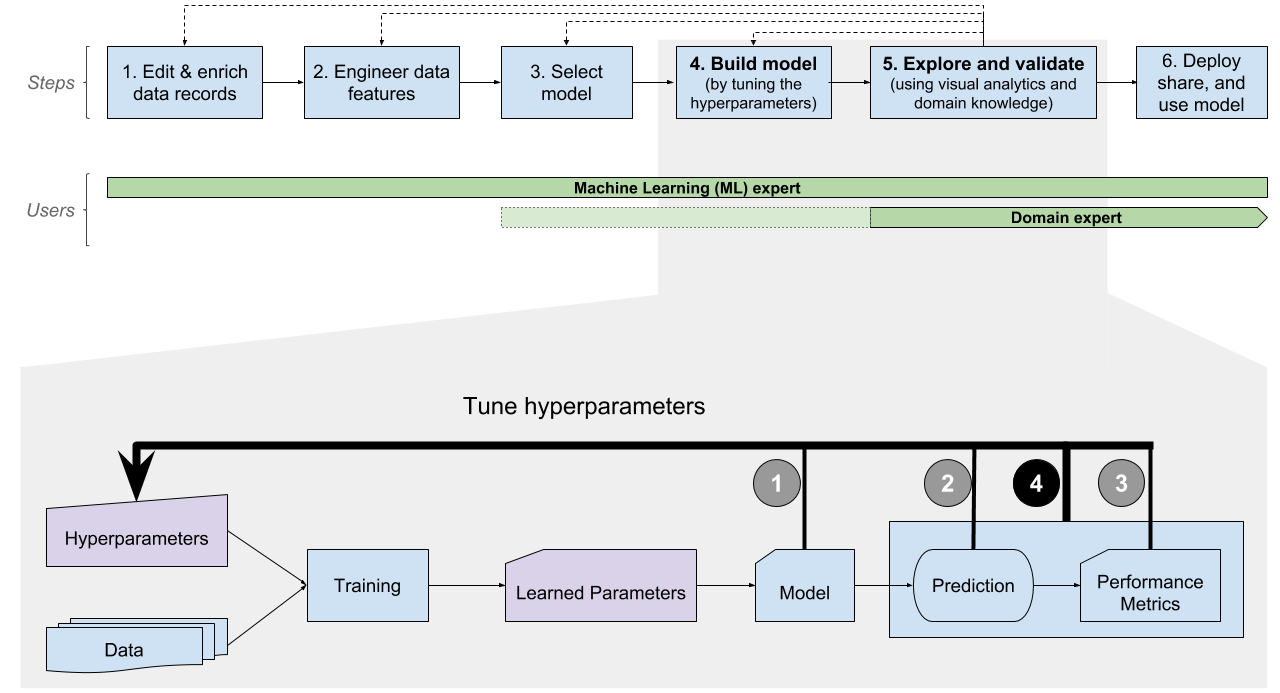
\includegraphics[width=\textwidth]{pictures/Figure1-Problem-In-Context}
 \caption{Problem in context. The top half (context): overall work process by a data science practitioner of addressing hard questions by applying an ML model to a dataset ~\cite{SachaHuman-CenteredChallenges}, p. 642. The bottom half (problem): model building via hyperparameter tuning and result validation.}
 \label{fig:Problem-In-Context}
\end{figure*}
\skye{The set of problems we focus on in this paper appears in the context of data science practitioners training a machine learning model to answer some questions regarding a dataset. For example, given all the customers of a company in the past 10 years, who are likely to extend their subscriptions, and who might cancel and leave? When building an ML model to make predictions on customer churn, the data science practitioners first acquire, clean, and enrich the customer data (Step 1 in the top half of Figure \ref{fig:Problem-In-Context}). Then they engineer the relevant features of the customers to be used in making predictions (Step 2 in the top half of Figure \ref{fig:Problem-In-Context}). They also need to select what ML model to use: more traditional models like a decision tree, or some complicated neural network models? (Step 3 in top half of Figure \ref{fig:Problem-In-Context}). While training the selected model, many models require hyperparameters that must be set and tuned. For example, a decision tree needs a criterion function (Gini index or entropy) to measure the quality of a node split, a maximum depth of the tree, and other hyperparameters. A neural network can have many hyperparameters such as the number of layers, which activation function to use, and so on (Step 4 in the top half of Figure \ref{fig:Problem-In-Context}). With the hyperparameters set, the models are trained and validated with a subset of the customer data (Step 5 in the top half of Figure \ref{fig:Problem-In-Context})}. If not satisfied, the data science practitioners iterate by returning to any of the prior four steps, depending on the results. Finally, when satisfied, they can share with other data analysts and domain experts or embed the model into a business process.
% e.g., the customer churn use cases where the questions are about identifying the top customers who are likely to extend vs. cancel their subscription with the company. 
% In the top half of Figure \ref{fig:Problem-In-Context} we summarize the work process via an adaptation of the pipeline described by ~\cite{SachaHuman-CenteredChallenges} (see Fig. 1 in ~\cite{SachaHuman-CenteredChallenges}, p. 642). It includes a few adaptations based on the authors' review of current tools and practices of data science practitioners. Consistently with the characterization by ~\cite{SachaHuman-CenteredChallenges}, the process starts with acquiring, cleaning, and enriching the data about the problem (step 1), continues with engineering the features that describe the problem (step 2), then once the data is prepared the ML expert selects the model (step 3), and builds it by tuning its hyperparameters (step 4). To evaluate the results of these four steps, the ML expert uses visualizations and domain knowledge (i.e., own knowledge or from interactions with the domain expert) (step 5) and, if not satisfied, iterates by returning to any of the prior four steps. Finally, when satisfied, s/he deploys the model. The model is typically shared with data analysts and domain experts who can use it or apply to similar data sets (e.g., domain experts and data analysts in sales or marketing may apply the model, deployed as an API, to score a new data sets of prospect customers and decide whom they should contact).

We focus on the problem of hyperparameter tuning: see steps 4 and 5 and the bottom half of Figure \ref{fig:Problem-In-Context}. 
% The bottom half of Figure \ref{fig:Problem-In-Context} characterizes more in detail these two steps. 
It's worth prefacing, first, the distinction between two types of parameters. The first is the \textit{hyperparameters}, which are set before the learning process begins by the users. The second is the \textit{learned parameters}, for example, "weights" of the data features the model learns from the dataset. The hyperparameters are the knobs with which human can steer the resulting model and performance.
% These are learned from the data to which the model is applied. They are typically derived by minimizing or maximizing a predefined objective function and are then applied as "weights" to the data features fed into the model. 
% Hereon we will call \textit{Learned parameters} the parameters the machine learns from the data and \textit{Hyperparameters} the parameters the ML expert tunes while building the model. 
% In this work, we focus on the latter. 
\gregorio{In the bottom half of Figure \ref{fig:Problem-In-Context}}, we indicate three leverage points to support hyperparameter tuning and, in this context, our focus in this paper.
% with the black arrow three types of support given by visual analytics tools to the ML expert as s/he decides what hyperparameters to use. 
The first is to visualize the model structure (e.g., what layer of the neural network model is processing what data features ~\cite{Liu2017TowardsPerspective}; see the vertical line with label 1). The second is to learn a local model around the model prediction (e.g., what features an image-recognition model leverages to classify a specific image ~\cite{Ribeiro2016quotWhyYouquot}; see the vertical line with label 2). The third is to algorithmically optimize hyperparameter values with an objective function.
% given both model prediction and, additionally, via aggregates performance metrics (e.g., precision, recall, accuracy, etc.; see the vertical line with label 3). }
\skye{In this work, we treat the model as a black box, and combine the second and third leverage points via interactive visual analytic to support hyperparameter tuning (see the vertical line with label 4).}

\section{Related Work}
% In this section, we first define the different types of parameters in machine learning, then we describe current support available in the model tuning from different perspectives.

% \subsection{Hyperparameter tuning}
% below are about parameter analysis, outdated
% \paragraph{Learned parameters} in most cases are \textit{weights} of feature functions. Visual analytics community has a long tradition in visualizing data features and/or machine learned weights of them to help users explore the data and adjust the learned weights. The visual parameter space analysis is an approach that maps \textit{parameter inputs} to the corresponding resulting \textit{output} to deal with the complexity of simulation models while still keeping human in the loop ~\cite{Sedlmair2014VisualFramework,Pretorius2011VisualizationAnalysis}.
% The recent development of human-in-the-loop research efforts unleashes a greater potential to interpolate human guidance in machine learning models. Visual analytics tools like StarSPIRE ~\cite{Bradel2014Multi-modelAnalytics} shield users from directly manipulating the parameters and instead interpret user insights via semantic interaction ~\cite{Endert2014TheAnalytics}. Andromeda brings human further in the loop~\cite{Self2016BridgingAnalytics} with object-level interaction (OLI) that generates new projections to reflect user interaction on data points.

% \paragraph{Hyperparameters} are all the parameters pre-determined by the user, including how the labelled data is split into training/validation/test sets, how much CPU memory is assigned, and most importantly, the model hyperparameters that configure various aspects of the learning algorithm. 

Hyperparameter tuning is an essential step that plays a big role in model performance. In order to get an ML model to work well in practice, the hyperparameters need to be tuned when training the model and the best settings usually differ for different datasets. Revising the configuration of existing learning paradigms can sometimes lead to more improvement in model performance than inventing new ones ~\cite{Pinto2009ARepresentation,CoatesAnLearning}. 
However, evaluating the effect of a given hyperparameter setting is expensive since it usually requires the model to be trained and tested, which is often computationally costly and may have random factors that make the evaluation even harder. 

\subsection{Visual Analytics Support in Parameter Search}
Exploring the relationships between several explanatory variables and one or more response variables has been a shared challenge in many different application domains, including meteorology \cite{Potter2009Ensemble-Vis:Data}, biology \cite{Pretorius2011VisualizationAnalysis} and medical science \cite{Afzal2011VisualEvaluation}. Statistical approaches such as the response surface methodology (RSM) \cite{BoxG.E.P.andWilson1992OnConditions} has been widely employed in developing solutions to those problems, and is further developed into the "design and analysis of computer experiments", and "visual parameter space exploration" \cite{Sedlmair2014VisualFramework} in the visual analytics community. Assessing the optimality of a black-box model often involves visualizing and sampling from multi-dimensional spaces, using surrogate and/or simulation models, contrasting the tradeoffs of several input settings, as well as understanding the influence of the inputs on the outputs. With these shared challenges, the frameworks and strategies developed for non-ML applications are generally applicable to hyperparameter tuning as well. For example, the four navigation strategies proposed by Sedlmair et al. \cite{Sedlmair2014VisualFramework} can also serve most of the exploration and analysis needs in the hyperparameter tuning process. However, hyperparameter tuning optimizes a machine learning model of  rather than the data itself. This extra layer of abstraction introduces additional challenges in comparison to non-ML problems. Users are required to make sense of the two-fold relationship: the hyperparameter settings, the  

Prior work on hyperparameter tuning, or hyperparameter search, can be broadly divided into two camps: automated approaches developed by the Machine Learning or AI researchers (e.g., see review in ~\cite{Claesen2014EasyOptunity}) and human-in-the-loop approaches developed by researchers working between Machine Learning and Visual Analytics (e.g., see review in ~\cite{SachaHuman-CenteredChallenges}), as the one proposed in this paper. Below we review these two camps of research.

\subsection{Automated Approaches} 
% In their review of this camp, 
Claesen et al. ~\cite{Claesen2014EasyOptunity} refer to the vision of a “fully automated, self-configuring learning strategy”, including hyperparameter search, as still the "holy grail of machine learning". Nevertheless, automatic approaches are showing increasing success on tuning hyperparameters of some models ~\cite{YogatamaEfficientTuning,Bardenet2013CollaborativeTuning}. Important contributions of the work done in this camp includes the formalization of key concepts (e.g., hyperparameter) ~\cite{Claesen2015HyperparameterLearning}, the identification of model tuning tasks that can be automated, and consequently software modules that implement specific hyperparameter optimization methods, such as Scikit-learn \cite{Pedregosa2011Scikit-learn:Python}, or packages that focuses on Bayesian methods (e.g., see https://bayesopt.github.io/), such as Hyperopt \cite{BergstraAlgorithmsOptimization} and ParamILS \cite{Hutter2009ParamILS:StutzleStStutzle}.
% or the packages that apply Bayesian methods (e.g., see https://bayesopt.github.io/) such as Hyperopt [Begstra et al. 2013] and ParamILS [Hutter et al. 2009]. 
On the commercial end of this camp, sample software tools include https://cloud.google.com/automl/ and https://www.datarobot.com/. 

While there are important advancements in the automated approaches camp, it's important to recognize that there are many practical scenarios where such automatic approaches are not applicable. An exhaustive \textit{grid search} is computationally expensive and time-consuming; \textit{random search} and surrogate-based model optimization require enough trials for a given dataset. Furthermore, implementing such an automatic approach usually require writing additional scripts and an in-depth understanding of the model, which excludes non-expert users of ML models or novice practitioners. 
As we learned in the interviews, the tuning process is either highly inefficient with manually keeping a notebook, or relies on automatic optimization algorithms that are usually expensive to implement without guarantee of success (convergence). Even when automated approaches are used, data scientists expressed a desire to combine both automated and manual iteration in one framework to help track of experiments and develop some intuition for potential modelling avenues to explore. In this article, we investigate where and how to leverage human guidance to improve the hyperparameter tuning efficacy.

\subsection {Human-in-the-loop Approaches}
The current reality of hyperparameter tuning is highly human-driven. Hyperparameter tuning is usually performed manually ~\cite{Claesen2015HyperparameterLearning} following rules-of-thumb and experience accumulated through practice ~\cite{Hinton2010AMachines,HsuAClassification}. Especially with complex models, the current trial-and-error process is inefficient in terms of the time spent and the computational load ~\cite{Pretorius2011VisualizationAnalysis}, and does not favor reproduceability, knowledge transfer, and collaboration (e.g., ~\cite{Claesen2014EasyOptunity}). To address these limitations, while increasing the transparency of ML models to humans, current research efforts in the human-in-the-loop camp have focused on three visual analytics foci: model structure, model prediction, model performance metrics.

\paragraph{Visualizing model structure.} Many visualization techniques have been developed to help users understand the structure of different ML models. 
Liu et al. ~\cite{Liu2016TowardsNetworks} developed a visual analytics system that shows all the layers, neurons, and other components of the convolutional neural networks, as well as how the training data is processed within. GANViz ~\cite{WangGANViz:Game} visualizes the adversarial training process of generative adversarial nets with linked coordinated visualizations. Rather than devoting to an in-depth understanding of a specific model, we investigate a more light-weight and general purpose support for model-agnostic hyperparameter tuning.

\paragraph{Interpreting model prediction.} There is an evolving research interest in model-agnostic interpretation, that focuses on understanding model prediction behaviors.
Riberio et al. developed LIME ~\cite{Ribeiro2016quotWhyYouquot}, a model-agnostic approach that learns an interpretable model locally around the prediction. This framework is extremely generalizable to different models and dataset, and efficiently enhanced the interpretability of a given model. However, before drilling down into such expensive interpretation and copious details, we focus on managing multiple models and support identifying better ones.

\paragraph{Interpreting model performance metrics.} The lack of support for evaluating the performance of ML models has been known for at least a decade now. For example, Patel and collaborators \cite{Fogarty2008CueFlik} in a 2008 study with data scientists observed that tuning ML models is an iterative and exploratory activity. It was hard for the data scientists in the study to track performance across iterations, which makes tuning process challenging. They argued that ML tools should include more suitable visualizations to help data scientists with their work. A recent attempt to provide more suitable visualizations of model evaluations metrics and model comparisons was made by Tsay and colleagues \cite{TsayRunway:Tool}. This is a research area that we expect will receive increasing attention in the near future.

\section{Hypeparameter Tuning Requirements}
In the first phase of the project, we interviewed data science practitioners in industry to investigate their hyperparameter tuning practice, as ML experts and as colleagues of domain experts with business needs and knowledge. In this section, we characterize the key steps of the process and user needs not yet addressed \skye{by current tools}.

\subsection{Method}
We interviewed six data science practitioners. While all were experienced in hyperparameter tuning, they held various job roles, including "data scientist", "data science engineer and researcher", "machine learning engineer", and "software engineer for a data analytics product". 
%On average, they had \textbf{k+} years of experience performing data science projects. 
We will refer to the six interviewees as Mk, Ch, An, Mc, Jm, and Ns. 

Our interviews may be affected by potential sampling biases: the interviewees were based in the United States and the UK; they worked for a software company that builds applications for large-scale enterprise machine learning and analytics. However, the sample included a good variety of job roles and, we believe, can represent the need of a broader range of data science practitioners in the industry (i.e., their colleagues and customers in other companies). In this first phase of the project, we aimed at a qualitative characterization of the hyperparameter tuning process and user requirements rather than quantitative findings.

The procedure of each interview followed a semi-structured method and included two sub-sessions. The first sub-session, lasting about 15 minutes, investigated the job role and working context of the interviewee:
\begin{enumerate}
\item Please briefly describe your job role.
\item Please describe the most common tasks for your job role.
\end{enumerate}
The second sub-session, lasting about 45 minutes, investigated the model tuning practices:
\begin{enumerate}
\item Please describe example projects, where you needed to train and tune models.
\begin{itemize}
\item What was your dataset, model and hyperparameters, evaluation metrics?
\item What do you look at to decide if the model can be better? What and how to tune?
\item How many experiments do you typically compare?
\end{itemize}

\item How would you perform the above task with other models? (generalizability of 1)
\item What kind of assistance would help you with the tasks you described?
\end{enumerate}
We asked follow-up questions depending on the interviewee's answers. In addition, we asked the interviewees to introduce us to the tools they use and, when possible, provide us with examples of their projects (e.g., outputs from hyperparameter tuning in a representative project, see Figure \ref{fig:realtable} and \ref{fig:train_histories}). Each interview was recorded and transcribed. 

Two of the co-authors performed a qualitative analysis on each transcript and summarized common themes (i.e., common steps, tools, and pain points). The themes were finally validated with other two co-authors, who are domain experts in data science tools. In the next two subsections we summarize the interview findings about the tuning practice and requirements, respectively.
\begin{figure*}
 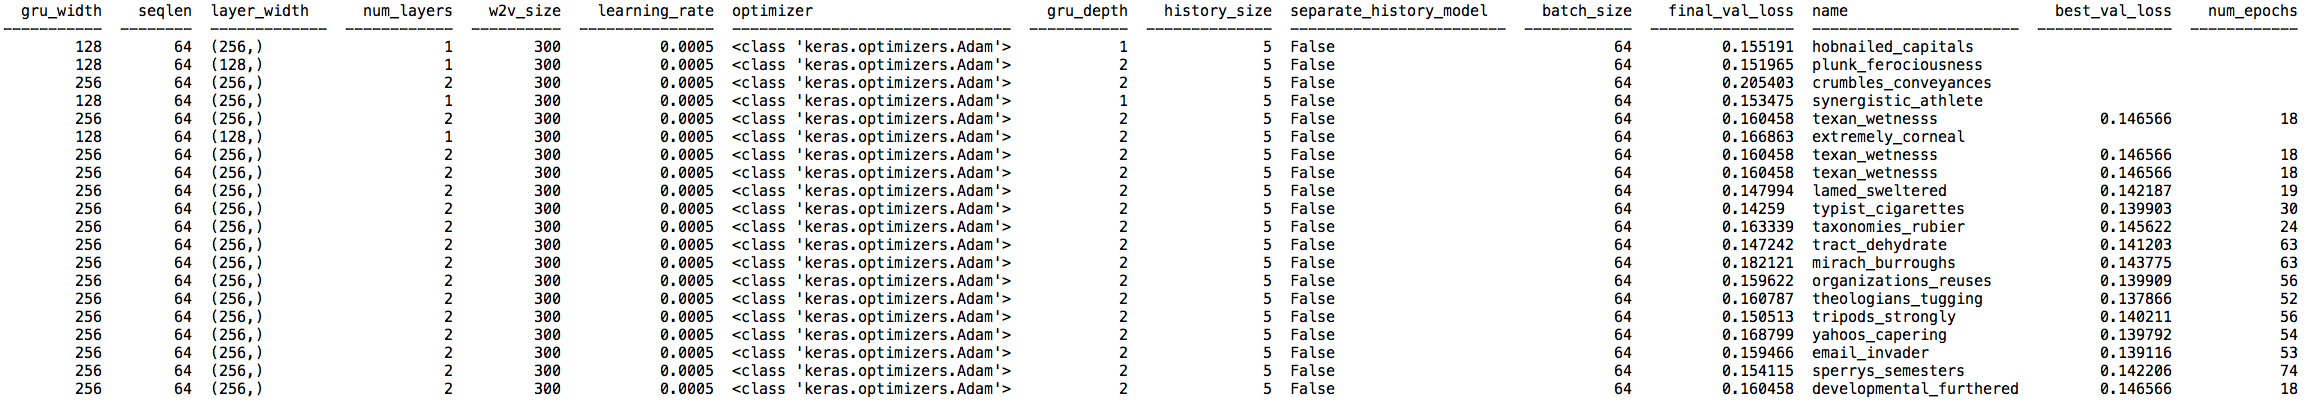
\includegraphics[width=\textwidth]{pictures/realtable}
 \caption{A text file showing some experiment history from Mc}
 \label{fig:realtable}
\end{figure*}
\begin{figure}
 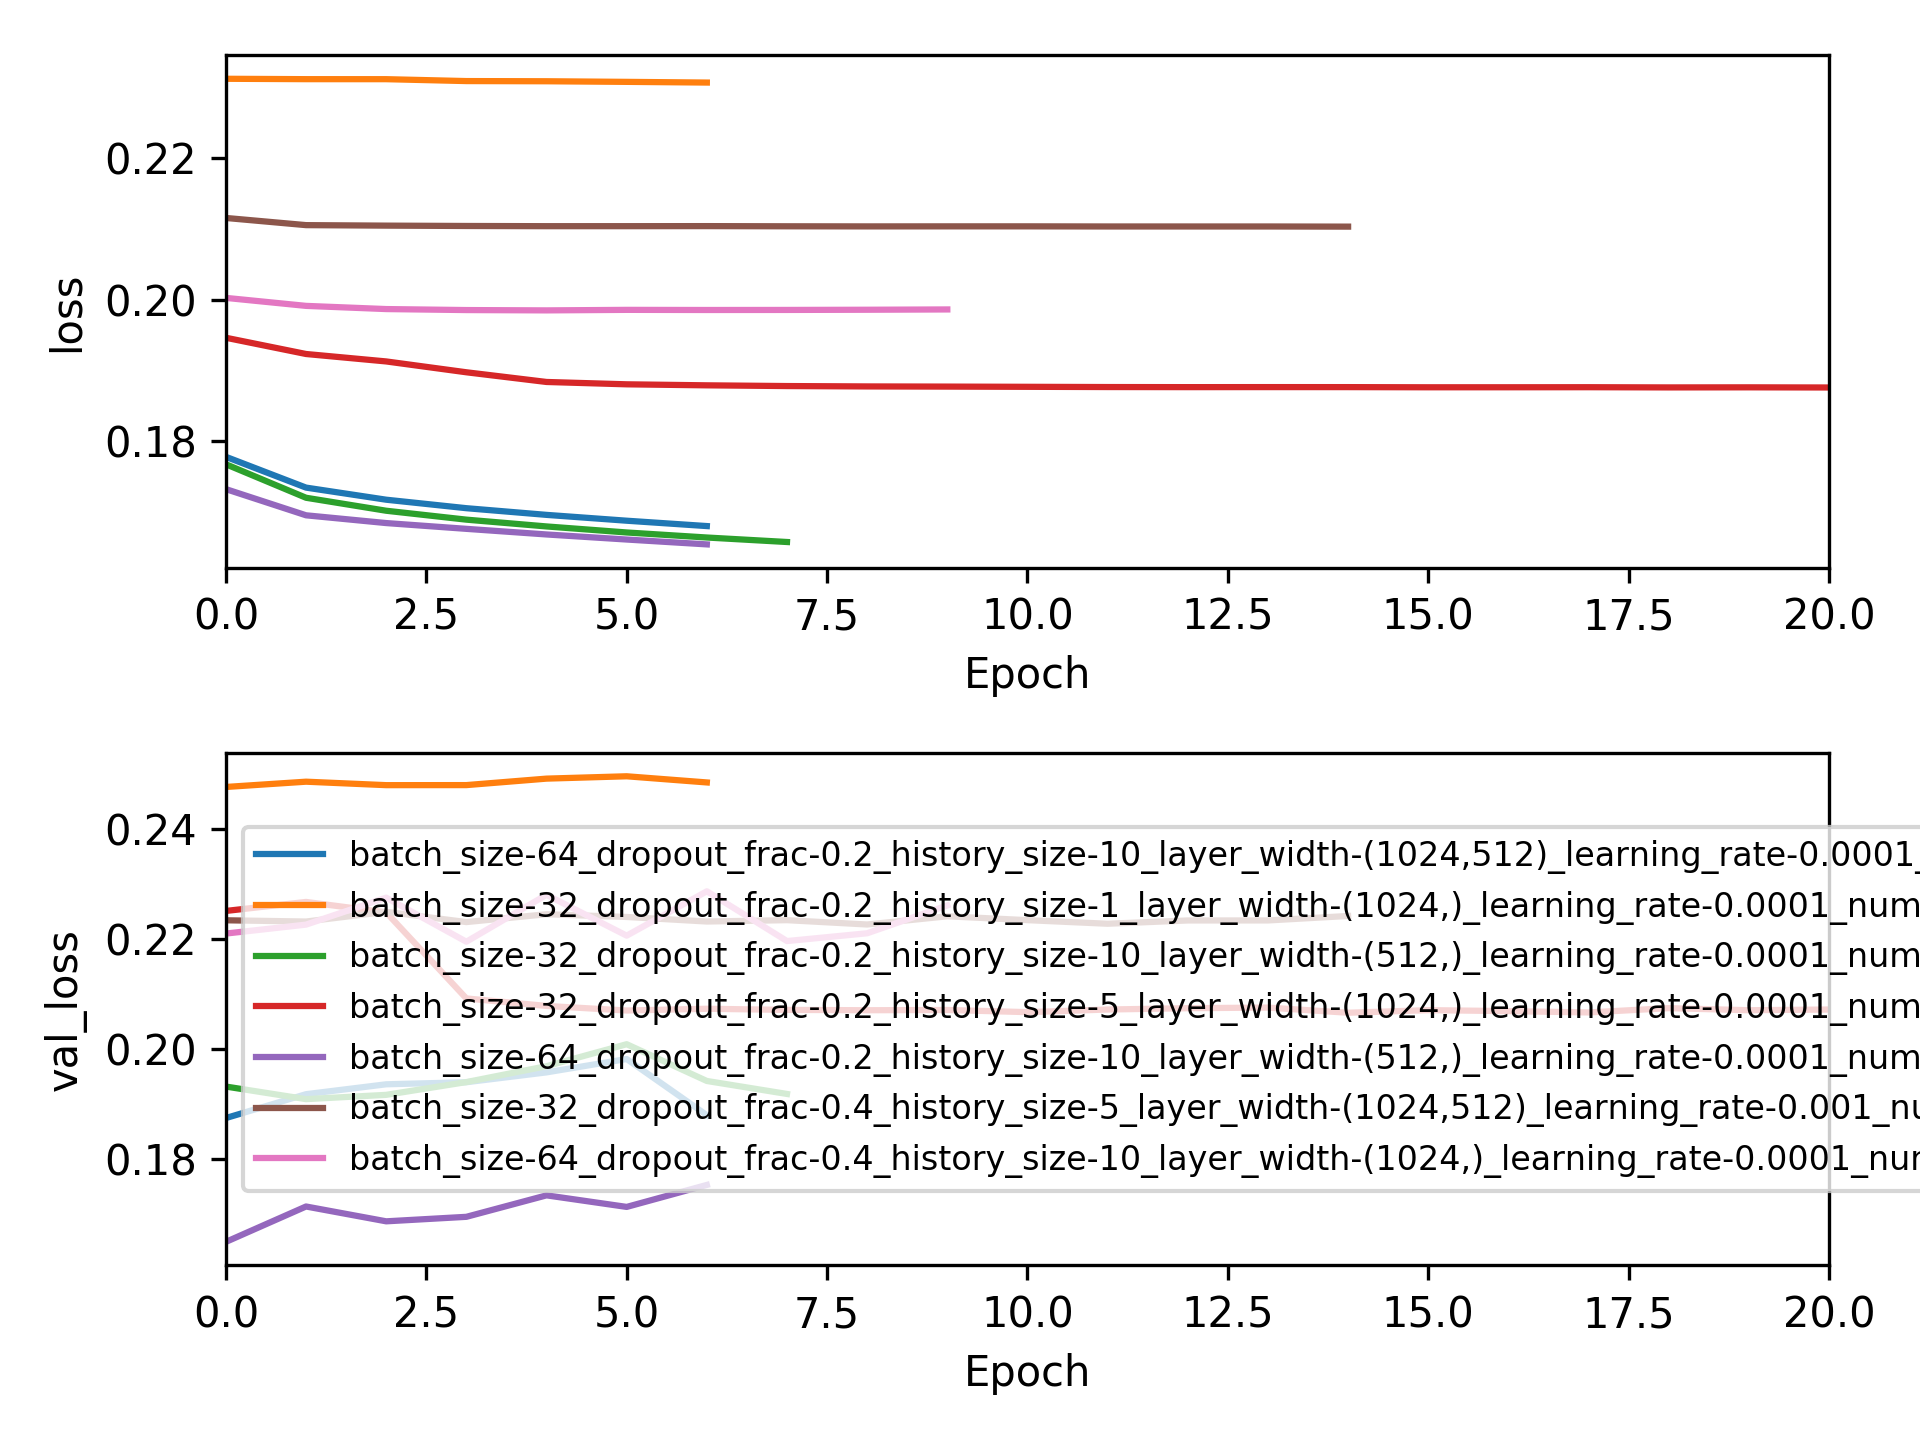
\includegraphics[width=\columnwidth]{pictures/train_histories}
 \caption{Example visualization example from Mc}
 \label{fig:train_histories}
\end{figure}
\subsection {Hyperparameter Tuning: Practice}
\subsubsection{How many tuning iterations or rounds do you do?}

The interviewees referred to a model tuning task as a project involving multiple experiments, which may last several hours or days. Two of the six data scientists (Ns and Mk) mentioned the strategy of starting from tuning simple models first (e.g., a logistic regression) and then, based on resources available (i.e., time and computation) vs. performance required, moving to tune more complex models. Generally, a model tuning project would require at least 20 experiments (Mk) and might take as many as about 60 experiments in the case of a deep learning model (Mc). This number could be significantly higher if parts of the tuning and experimental process were automated.
% \begin{itemize}
% \item Mk: at least 20 experiments, for a model tuning project.
% \item Mc: about 60 experiments to tune a deep learning model.
% \item The interviewees referred to a model tuning task, involving multiple experiments, as a project which may last several hours or days. About the longer-term context of tuning a specific model, two of the six data scientists (Ns and Mk) mentioned the practice of starting from tuning simple models first (e.g., a logistic regression) and then, based on resources available (i.e., time and computation) vs. performance required, moving to tuning more complex models.
% \end{itemize}
\subsubsection{What hyperparameters do you tune? How?}
The number of hyperparameters differs model by model. In the case of a deep learning model, there are often dozens of hyperparameters. 
% common examples are the number of layers, dense or recurrent networks, width of each layer (i.e., how many neurons per layer), learning rate, the optimizing algorithm, and how much dropout to use. 
% \tristan{(Tristan: this seems too high. I'd say "often dozens")} 
The interviewees would focus on tuning \textit{"a dozen or more" (Mc)} hyperparameters. It usually relies on the data science practitioners to plan and \textit{"keep everything as a changeable parameter or knob" (Mc)} in their code.

The data science practitioner who shared the Figures \ref{fig:realtable} and \ref{fig:train_histories} describes his typical hyperparameter tuning process below. 
Not all hyperparameter values need to be tuned, such as the learning rate. Some commonly tuned hyperparameters include the optimizing algorithm, dropout rate, the number of layers, the width of each layer, to name just a few. \textit{"I do not really try to fix those right off the bat. Instead, I define limits, so I bound what values I think they could take, and then I either do a grid search or a random parameter search"}. In the example project Mc described to us, it usually takes about 6 hours to train a model with one set of hyperparameters. In addition, there's only a certain amount that can be parallelized due to the limited CPU resources. In such situations, random parameter searches are more commonly used because the results would converge faster, and provide a better sense of the hyperparameter space.

When deciding if a specific hyperparameter should be tuned more, Mc usually \textit{“hold all other features constant [across experiments], and just experiment with one."} If the results do not change much, this hyperparameter might not be worth further tuning. For example, a lot of people find learning rate not very important to affect their results. It is useful to figure such things out sooner, to eliminate hyperparameters that do not need to be tuned anymore.
% \begin{itemize}
% \item About the number of hyperparameters managed in a project. Mc: "a dozen or more" hyperparameters for a deep learning model. On deep learning models: \textit{"The model itself has a lot of hyperparameters. Even just the structure of the model is a hyperparameter. So when I create the code to train the model I keep everything as a changeable parameter or knob." (May 23, 2018).} About examples of hyperparameters tuned for these models, some pertain to the model structure, such as the number of layers, dense or recurrent networks, width of each layer (i.e., how many neurons per layer), learning rate, the optimizing algorithm, and how much dropout to use.
% \item About the tuning practice. The data science practitioner who shared the Figures \ref{fig:realtable} and \ref{fig:train_histories} describes what hyperparameters he tunes and how: \textit{“There are ones [or hyperparameters] that I don’t even try to fix, for example, what my learning rate is. [Other hyperparameters I tune are] the optimizing algorithm I use, how much dropout should I use, if I have two or three layers of my internal [network] (like decoder or encoder), are they dense networks or they are recurrent networks, […] what’s the width of each one of those layers (like how many neurons should they have). I don’t really try to fix those right off the bat. Instead, I define limits, so I bound what values I think they could take, and then I either do a grid search or a random parameter search. Grid searches are nicer, I’d prefer doing those but they are very time-consuming, so for this model before I did a bunch of optimizations and restricting the size of the neural network and all that. It took about 6 hours to train on one set of hyperparameters, and we only have 2 GPUs in-house so there's only a certain amount that we can parallelize that so generally I prefer doing random parameter searches because you converge faster, gives you a better sense of what's going on.”} Interviewer: "How do decide if a specific feature [hyperparameter] should be tuned?". Mc: \textit{“You basically hold all other features constant [across experiments], you just vary that one, and you see if the results are changing. [...] For example, a lot of people find in a lot of practical models that learning rate does not affect their results that much. So finding that out soon is useful because it removes a whole variable that you do not need to tune anymore”.}
% \end{itemize}
\subsubsection{What performance metrics do you track? How?}
The commonly used performance metrics for supervised models include accuracy, precision, recall, and ROC curves. Other examples are learning curve (to check the slope of that line and when it gets saturation), training loss vs. validation loss (to check when the latter increases as the first keeps decreasing to detect overfitting). 
% \begin{itemize}
% \item Jm: for common supervised models, for example, accuracy, precision, recall, ROC curves.
% \item Mc: learning curve (checking the slope of that line and when it gets saturation), training loss vs. validation loss (checking when the latter increases as the first keeps decreasing - model overfit) 
% \end{itemize}
\subsubsection{Workflow}
The six data science practitioners pointed to a similar underlying process of hyperparameter tuning. What we learned was consistent with the reports from the literature about the general process, which we summarized at the top of Figure \ref{fig:Problem-In-Context}. An interviewee (Mk) summarized the process as follows:
% For example, Mk describes this general process as follows: 
\textit{"We go through a typical data science workflow, which is clean data, train a model, and then open it up over an API to a web front-end.".} 
In addition, our interviews allowed us to characterize hyperparameter tuning in more detail. 
% This part of the process corresponds to steps 4 and 5 described at the top of Figure \ref{fig:Problem-In-Context}. 
% The six interviews led us to characterize this part, the hyperparameter tuning workflow, as consisting of five sub-tasks, with the first four forming a loop. We describe it in Figure \ref{fig:workflow} and the paragraphs below. 
We formalize the hyperparameter tuning process as a workflow with five sub-steps (shown in Figure \ref{fig:workflow}), with the first four forming a loop. 
\begin{figure*}
 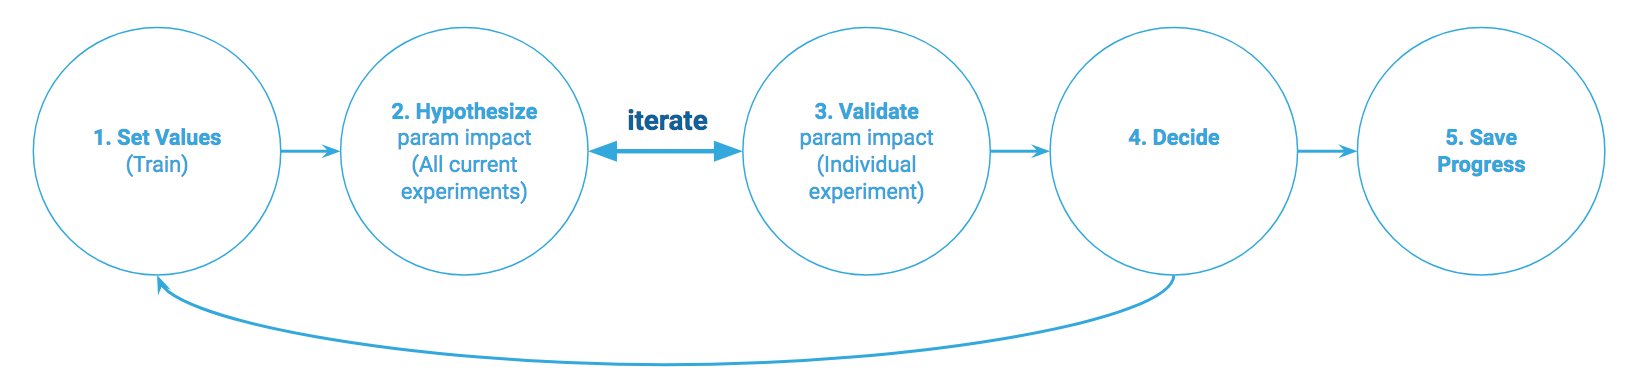
\includegraphics[width=\textwidth]{pictures/workflow}
 \caption{Formalized workflow of the hyperparameter tuning process.}
 \label{fig:workflow}
\end{figure*}

\paragraph{Sub-step 1: Set hyperparameter values.} At the outset of the workflow (the leftmost circle in Figure \ref{fig:workflow}), the ML experts initiate the first batch of experiments by setting hyperparameter values based on their understanding of the data, the model, and the problem to solve. This sub-step reoccurs later as a restart of the loop if, after sub-step 4 (the fourth circle in Figure \ref{fig:workflow}), the ML expert decides that more tuning is still needed. 
% 3) How close is our recommendation for my decision?
% When it occurs at the very beginning of a hyperparameter tuning project, the answers to the questions are based on the practitioner's prior experience with the model and ML data. 
% When it re-occurs later the practitioner answers the questions by relying on the support such as the history of hyperparameter value combinations (i.e., experiments) run and their respective results. 

\paragraph{Sub-step 2: Hypothesize the impact of tuned hyperparameters with results of all experiments.} At this stage the ML expert has just run a batch of experiments and wants to answer two questions: 1) What are the most impactful hyperparameters in these experiments? Is hyperparameter X relevant?
% (most unsure, why is this not yet a production model?) 
2) How do the hyperparameters influence the performance of the model and what performance metrics to consider? 
% Is it obvious what to do next? 
This sub-step is performed with the support of summative reports of the hyperparameters and performance metrics for a full batch of experiments.

\paragraph{Sub-step 3: Validate hypotheses with details of individual experiments.} While the ML expert is testing some general hypotheses in the previous step, s/he may need to drill into the details of specific experiments: 
% 1) Why are the parameters influencing the performance the way they do? 
1) What do the details of this experiment say about my hypotheses? 2) Do I trust the predictions of this models by looking at the results?
This sub-step represents an in-depth investigation that starts and ends back in sub-step 2 (see bidirectional arrow in Figure \ref{fig:workflow}). It is performed with the support of detailed reports on hyperparameters and performance metrics from an individual experiment. Multiple micro-iterations occur between sub-steps 1 and 2, typically.

\paragraph{Sub-step 4: Decide if more tuning is needed.} Once the ML expert has gathered the evidence from the current batch of experiments then he decides: 1) Does the (best) model performance meet my expectations? 2) If not, will more training improve the model performance and will it be worth the efforts, given the resources?
This sub-step is performed with the support of the summative and detailed reports from the prior two steps
% plus a history of what combinations of hyperparameters values have already been explored earlier and with what general results.

\paragraph{Sub-task 5: Review progress and Save Progress results.} If the ML expert decides, in sub-step 4, that no more tuning is needed, then he answers these questions: 1) How well am I able to recall the tuning process and communicate its results? 2) How useful are the records of my tuning progress? What is missing? What is superfluous? 
This sub-step is performed with the support of a final project-level report summarizing all the experiments from all batches plus any comments or reminders the practitioner recorded during the tuning process.

\subsection{Hyperparameter Tuning: Support Needed}
Following the workflow in Figure \ref{fig:workflow} we identified at each step needs for visual analytics support that are not fully addressed by current data science tools.

\subsubsection{Analytics of batches of experiments}
One of the most evident needs emerging from the interviews is the need for visualizations that aggregate results across experiments and allow group-level comparisons among the experiments in a batch. 
% A batch represents a subtask or iteration in the larger hyperparameter tuning task. 
The data science practitioners need visualizations that help to efficiently make sense of experiment results and determine what hyperparameters values are satisfying and what values are not and thus requiring more exploration. They also need to interactively customize the visualization. In the words of an interviewee (Ch): \textit{"Visualization is to bring human interpretation in hyperparameter tuning... build a visualization that is a natural interpretation of the actual data passed in, ... Users always want variation, they should be allowed to customize the visualization"}. Currently, these visualizations are created manually and in ad hoc fashion. A data science practitioner (Mk) summarize his current practice as follows: \textit{"You try different combinations of hyperparameters, keep track of the performance, and visualize it somehow"}.   

\subsubsection{Analytics of individual experiments}
A second general need is a support to investigate results and metadata of an individual experiment. As shown in Figure \ref{fig:workflow}, these investigations happen as drill-down iterations in the broader context of making sense of the entire batch of experiments and testing the current working hypotheses. 
% Most commonly, the analysis is done after the experiment is completed. 
For example, the user may need to understand what happened in this experiment and if the model predictions can be trusted. Additionally, s/he may want to review the metadata as a reminder of the hyperparameter values used and even annotate any notes from the analysis if the experiment is worth tracking for later comparisons. In particular, three of the six practitioners (Ns, Mk, Mc) mentioned the need to review interpretability details such as examples of misclassifications by a supervised ML model. Mk: \textit{"Interpretability is also an important factor to track when turning hyperparameters. Is it predicting the right class for the right reason? I would want to get examples which get classified correctly or not."} ~\cite{Ribeiro2016quotWhyYouquot}.

With computationally expensive experiments that may take hours, analysis of an individual experiment is very desirable also before completion. Two interviewees explicitly pointed to the need for "early stopping" (Mk) of ineffective experiments. Mk: \textit{"If I see the loss curve jumping all over the place, or very noisy in comparison to the other loss curves, I don't even need to ever look at that model again, I just thought it out immediately"}.
% (May 23, 2018).

\subsubsection{Informing the next round of exploration}
A third general need revolves around the support for making complex decisions. The decision is whether to run a new batch of experiments and, if so, what new set of hyperparameter values to use, given the results of the current batch of experiments. One of the challenges is to monitor and reason about many hyperparameters at the same time. This is particularly evident when training deep learning models. The data science practitioners have to restrict the number of variables to keep in mind due to limited cognitive capacity. When deciding what small subset of the hyperparameter space to explore next, they need to capture the insights from the analysis of the existing experiments (see the first two needs, above). It is worth remarking, about this need, that the decision consists in balancing observations, expectations, and resources: i.e., the performance observed in the current batch of experiments (observations), the desired level of performance given the problem (expectations) and the resources such as time and computation available to the project (resources). While the first is in the tool, the second and third are mostly in the head of the data science practitioner - herefrom the need for visual analytics tools that involve the human. As summarized by Mc: \textit{"There's never been a point in any project I've ever worked on where hyperparameter tuning was done. It's really just I [judging if] I have seen enough and I'm willing to make a decision about what the hyperparameter should be [to meet expectations]. So it’s more of a question of timelines and schedules"}.

\subsubsection{Project-level memory and communication}
The fourth need pertains to memory and communication support at the project level. About memory support, Jm describes the needs to capture what was done to easily recall it later: \textit{"Now in the report, we have the accuracy (performance), but we do not capture what I changed. Over time we will probably forget what we’ve done, such as the numbers we have changed, so being able to track them is important, we will be able to go back and see how the model has improved. [A] “rewinding” [capability]."}
Several interviewees (e.g., Ns, Mk) also mentioned that a project-level summary or report on all experiments should allow filtering, annotating, and comparing experiments: e.g., delete or archive experiment, mark as promising, filter, annotate or tag, select and compare two experiments. For example, Mk reports that his current practice is to compare two experiments at a time, in detail. Ns reports that, at the end of her tuning project, she typically selects the best 2-3 experiments from the list and then runs their models onto an entirely new dataset, as a final \textit{"blind validation"} step. 
Some interviewees suggested that project-level reporting would help collaborate with colleagues and communicate the results to the domain experts who requested the model. In Jm's words, \textit{"to be able to communicate to the business sponsors outside our team how well the model is performing, and also, we would use it internally for [guiding future] tuning [...] [and] do a comparison between models as well"}. 

\section{HyperTuner Prototype and Evaluation}
\begin{figure*}
 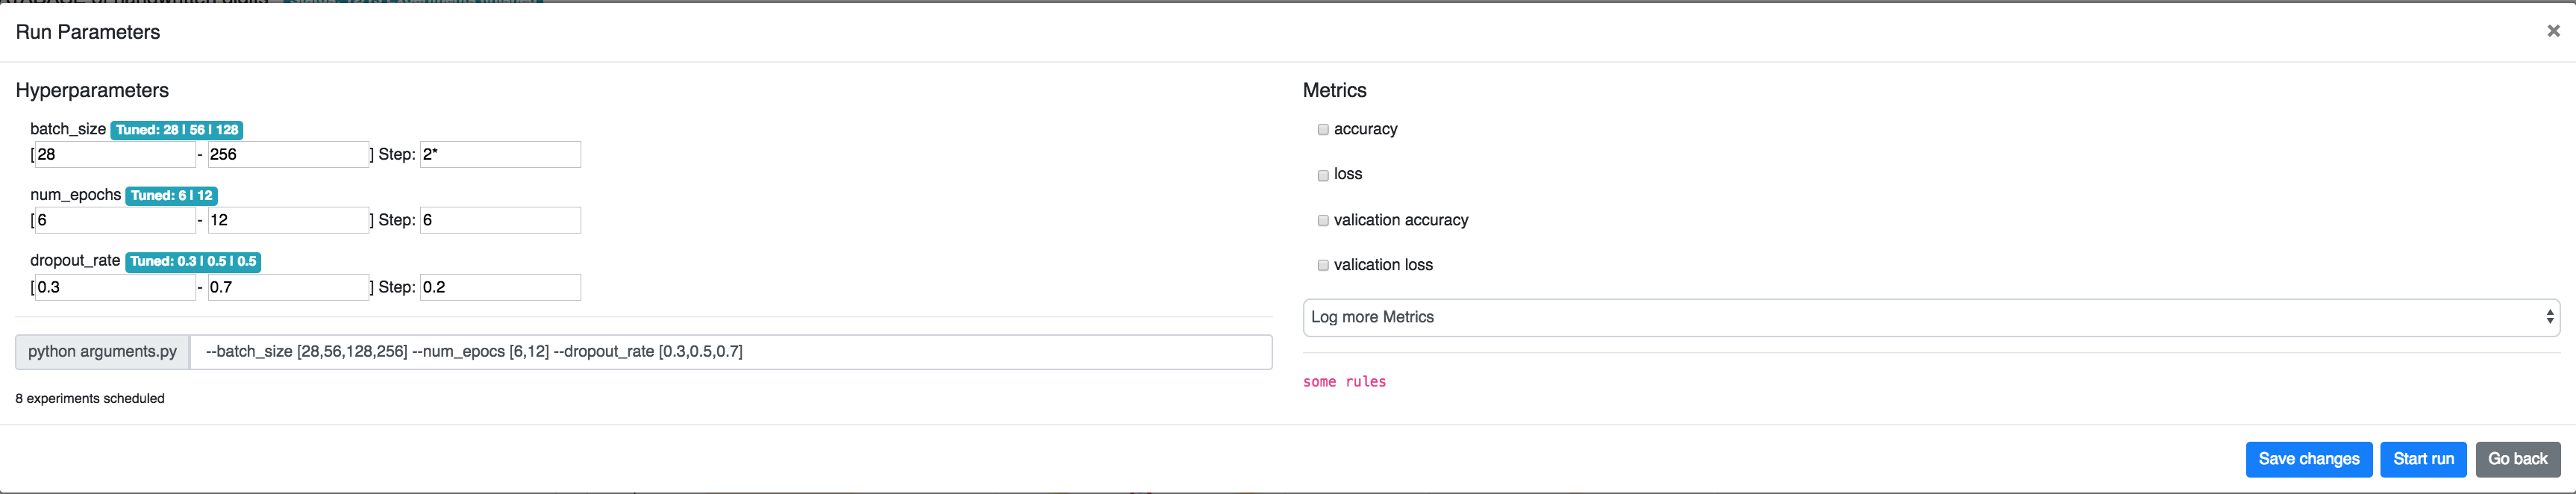
\includegraphics[width=\textwidth]{pictures/start}
 \caption{Initial Parameter Setting to Launch Experiments}
 \label{fig:start}
\end{figure*}
\begin{figure*}
 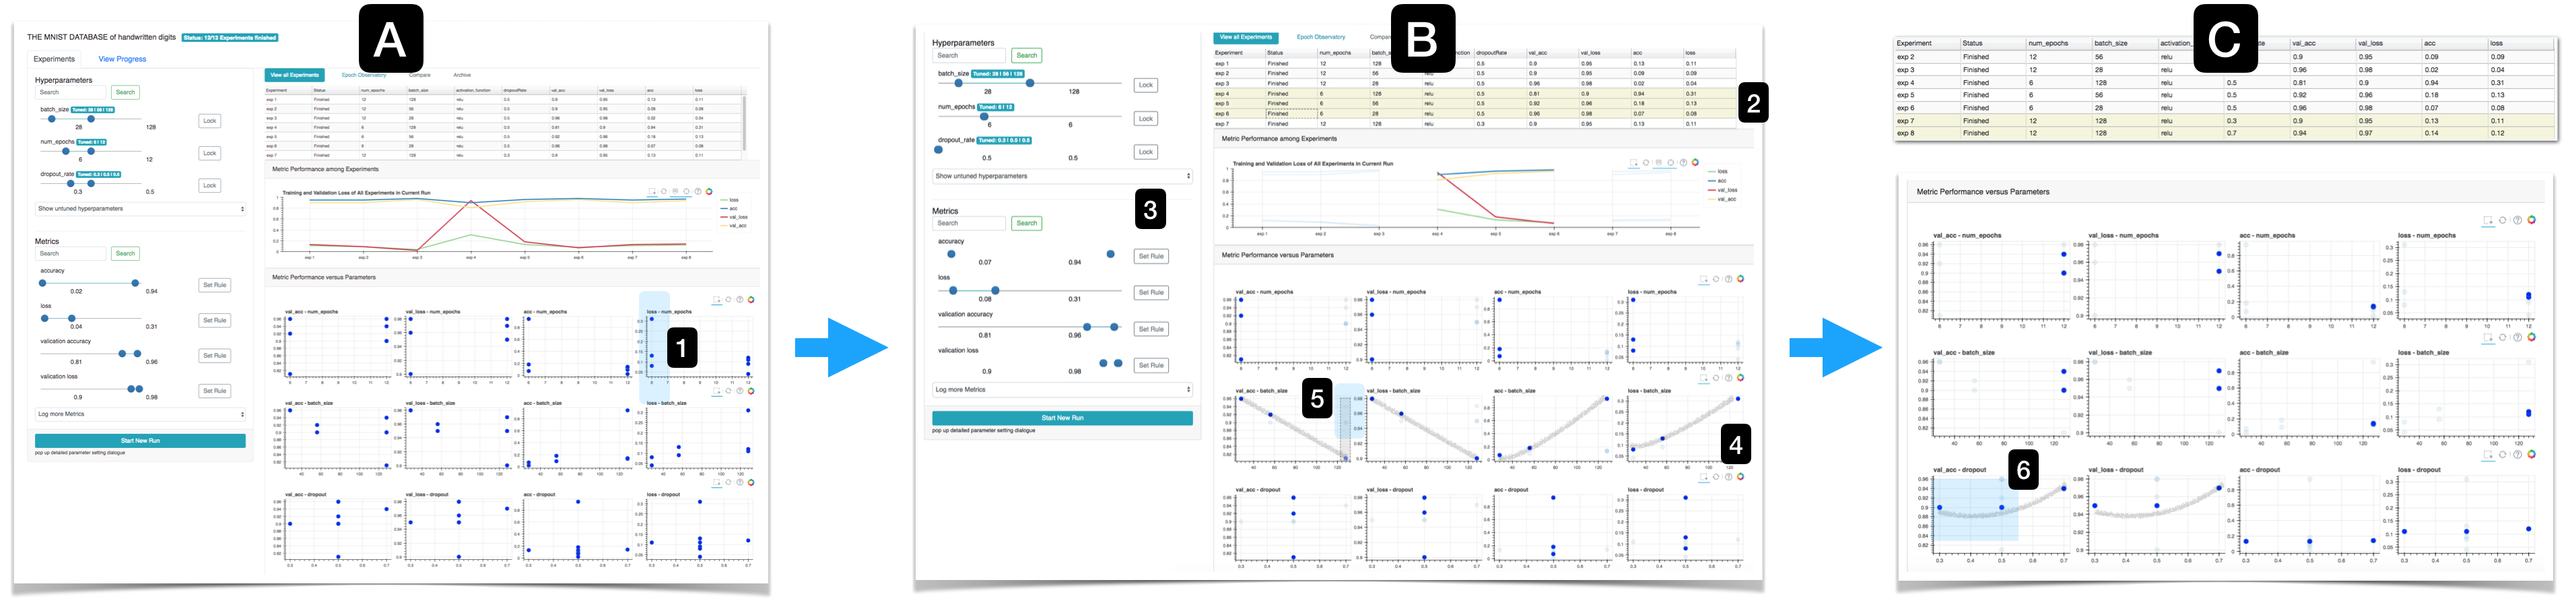
\includegraphics[width=\textwidth]{pictures/global}
 \caption{Run dashboard for a batch of experiments in an example interaction flow}
 \label{fig:global}
\end{figure*}
To explore how visual analytics tools can better support the hyperparameter tuning workflow (Figure \ref{fig:workflow}), we implemented and evaluated HyperTuner, an interactive prototype. 
\subsection{Implementation and Example Data}
HyperTuner is a web-based application implemented on the Django framework ~\cite{TheDjango}. The visualization components are developed with Bokeh ~\cite{WelcomeDocumentation} and D3.js ~\cite{D3.jsDocuments}.

\paragraph{Core Concepts in the Prototype.}
In the prototype, a \textsf{Run} represents a batch of \textsf{Experiments}. A run results from a user launching a training script on their personal computer or a remote compute environment. After launching a run, typically users have limited control beyond interrupting the entire run or interrupting sub-tasks if the run leverages multiple processes.

The user interactions supported around a specific \textsf{Run} correspond to completing a full loop connecting the first four sub-steps of the workflow in Figure \ref{fig:workflow}. To start a run, the user sets a list of values she wants to try for each hyperparameter and launches experiments with all combinations of the selected hyperparameter values. Each experiment consists of the same model \skye{skeleton (implemented in a script with hyperparameter as tunable variables)} and are trained on the same dataset. Once the experiments are completed, the prototype reports and visualizes the values of the performance \textsf{Metrics} obtained from each experiment with respect to the corresponding hyperparameter value settings. The user typically completes multiple runs until satisfied by the results, then selects the best models and reports these as the outcome of the entire model tuning \textsf{Project}.

\paragraph{Prototype Content and Use Cases.}
The design of the prototype is model-agnostic so that it can be applied to different models (see core concepts above). However, to demonstrate the prototype with real-world use cases, we run a real model tuning project and populated the visualizations with realistic data. Specifically, we built a simple convolutional neural network (CNN) and applied it to predict the MNIST dataset of handwritten digits ~\cite{MNISTBurges}. As a proof of concept, we streamlined a training set of 60,000 examples and a test set of 10,000 examples. 

Based on the data obtained from training the CNN model with 8 experiments, below we describe the prototype implementation through the following use case with two phases: 

Sarah is a data scientist and she is building a 10-way classifier with the CNN model to recognize the handwritten digit numbers in the MNIST dataset. She has implemented the model skeleton in a python script with the hyperparameters as tunable variables, and needs to decide what values to use.
\begin{itemize}
\item[] Phase 1: Sarah sets a list of values for each hyperparameter and launches a batch of \textsf{Experiments} in the current \textsf{Run}. After obtaining the training results, she makes sense of these results and decides how to continue the tuning process. 
\item[] Phase 2: Sarah stops the tuning progress, cleans up the training records, and saves her progress as a report.
\end{itemize}

\subsection{Phase 1}
\paragraph{Set Value to Launch Experiments.} Sarah started by experimenting with three hyperparameters: \textit{batch size (number of samples that going to be propagated through the network)}, \textit{dropout rate (the probability at which randomly selected neurons are ignored during training)}, and \textit{number of epochs (one epoch is when an entire dataset is passed forward and backward through the neural network once)}. She sets several candidate values for each of the three hyperparameters (Figure \ref{fig:start} left) and sets the remaining hyperparameters as default values. Notably, by adding an asterisk (*) after the step size she indicates that the step size increases by multiplying the previous value by two rather than adding two each time (e.g. 28,56,128 instead of 28,30,32). Then she selects the metrics she wants to use to measure the model performance (Figure \ref{fig:start} right). 
In response of her parameter setting actions, the tool automatically generates the command to execute the script via a command-line interface, which she commonly uses to run scripts (see the bottom left field in Figure \ref{fig:start}). She can further customize and add more hyperparameters in the final command, and choose to log more performance metrics (the bottom right drop-down menu of Figure \ref{fig:start}).

\paragraph{Run Dashboard.} After the experiments are launched and completed, Sarah reviews the results of all the experiments summarized in the run dashboard (Figure \ref{fig:global}(A)). By viewing the parameter panel on the left she is reminded of the hyperparameters values she had set when she launched this run plus the metrics she selected to assess performance. For each hyperparameter and metric, she can scan the current value ranges under each slide bar. On the right, she sees both the table and a set of visualizations. The experiment results are summarized in the table at the top: it lists experiment ID, status, hyperparameters tuned, and performance metrics obtained. Under the table, she finds two types of visualizations. The first is an aggregated line chart showing the performance metrics (lines) obtained for each of the eight experiments (x-axis). She can click on the legend to choose which performance metric to view. The second is a grid of 12 scatter plots (three rows, four columns) showing the detailed results for each metric-hyperparameter combination: each row corresponds to one hyperparameter (always shown on the x-axis) and each column corresponds to one performance metric (always shown on the y-axis).

Sarah notices that experiment 4 has worse performance than the others. She suspects that it's because this experiment had a low number of epochs. So by brushing over the top right scatterplot, she selects the experiments with the smaller number of epochs (num\_epochs=6, Figure \ref{fig:global} A.1) to see how these experiments performed (number of epochs corresponds to the first row). Since all views in this dashboard are coordinated, the brushing operation results in selecting three experiments across all views, including the table at the top (Figure \ref{fig:global} B.2). It also results into updated sliders in the parameter panel on the left: the lower and upper limit of each range (blue circles) in each slider is automatically re-positioned to reflect the hyperparameter and performance metrics of the experiments selected by the brushing (Figure \ref{fig:global} B.3). At this point, Sarah notices that as the experiments selected have num\_epoch=6 and dropout\_rate=0.5, the batch\_size shows a linear relationship with all the performance metrics (the relationship is highlighted for the reader with gray lines in Figure \ref{fig:global} B.4). Thus she infers that experiments with higher batch\_size values might have higher accuracy and lower loss values. Based on this insight, Sarah now selects the experiments with the largest batch\_size, batch\_size=128 (Figure \ref{fig:global} B.5). Based on this selection she has now identified three experiments (Figure \ref{fig:global} C), and it seems that dropout rates 0.3 and 0.5 are not as good as 0.7 (Figure \ref{fig:global} C.5). Yet, none of the three experiments has good accuracy, thus she decides to check each experiment in more detail via the experiment dashboard.

\paragraph{Experiment Dashboard.} Sarah clicks on the \textit{Epoch Observatory} sub-tab and enters the experiment dashboard, where the left panel and table at the top are persisted from the run dashboard where she was earlier. Here, in the table, she selects one of the three rows (experiments) she is investigating. She replays the training process of the individual experiment (Figure \ref{fig:local} label 1). She repeats this process with the other two experiments. She is investigating how the loss and accuracy curves look like in each experiment, and specifically, each epoch. This will help her find a good trade-off between good final performance and amount of noise (i.e., metric fluctuations) in the training process. In the experiment dashboard, under the table, she analyzes the configuration summaries or metadata of the experiment (label 2), the line charts showing the performance metrics (lines) within epoch (label 3) and across epochs (label 4). In each of these line charts, she clicks on the legend to choose which performance metric to view. On the lower right, she finds a visualization that is specific to the current model and dataset. In this case, she sees a confusion matrix as a heat map. This visualization helps her assess if she can trust the model trained in the current experiment. Specifically, she inspects the cells that show what digits are more frequently misclassified and why by looking at the examples shown, upon cell hovering, under the matrix. For example, she hovers over row 2 and column 6 and finds out that there are 14 data points that are actually digit "2" but classified as digit "6" (see frequency 14 in the matrix, magnified in Figure \ref{fig:local} label 5), and the images at the bottom are examples of those misclassified data points. This gives her a sense of the quality of the model predictions.
\begin{figure}
 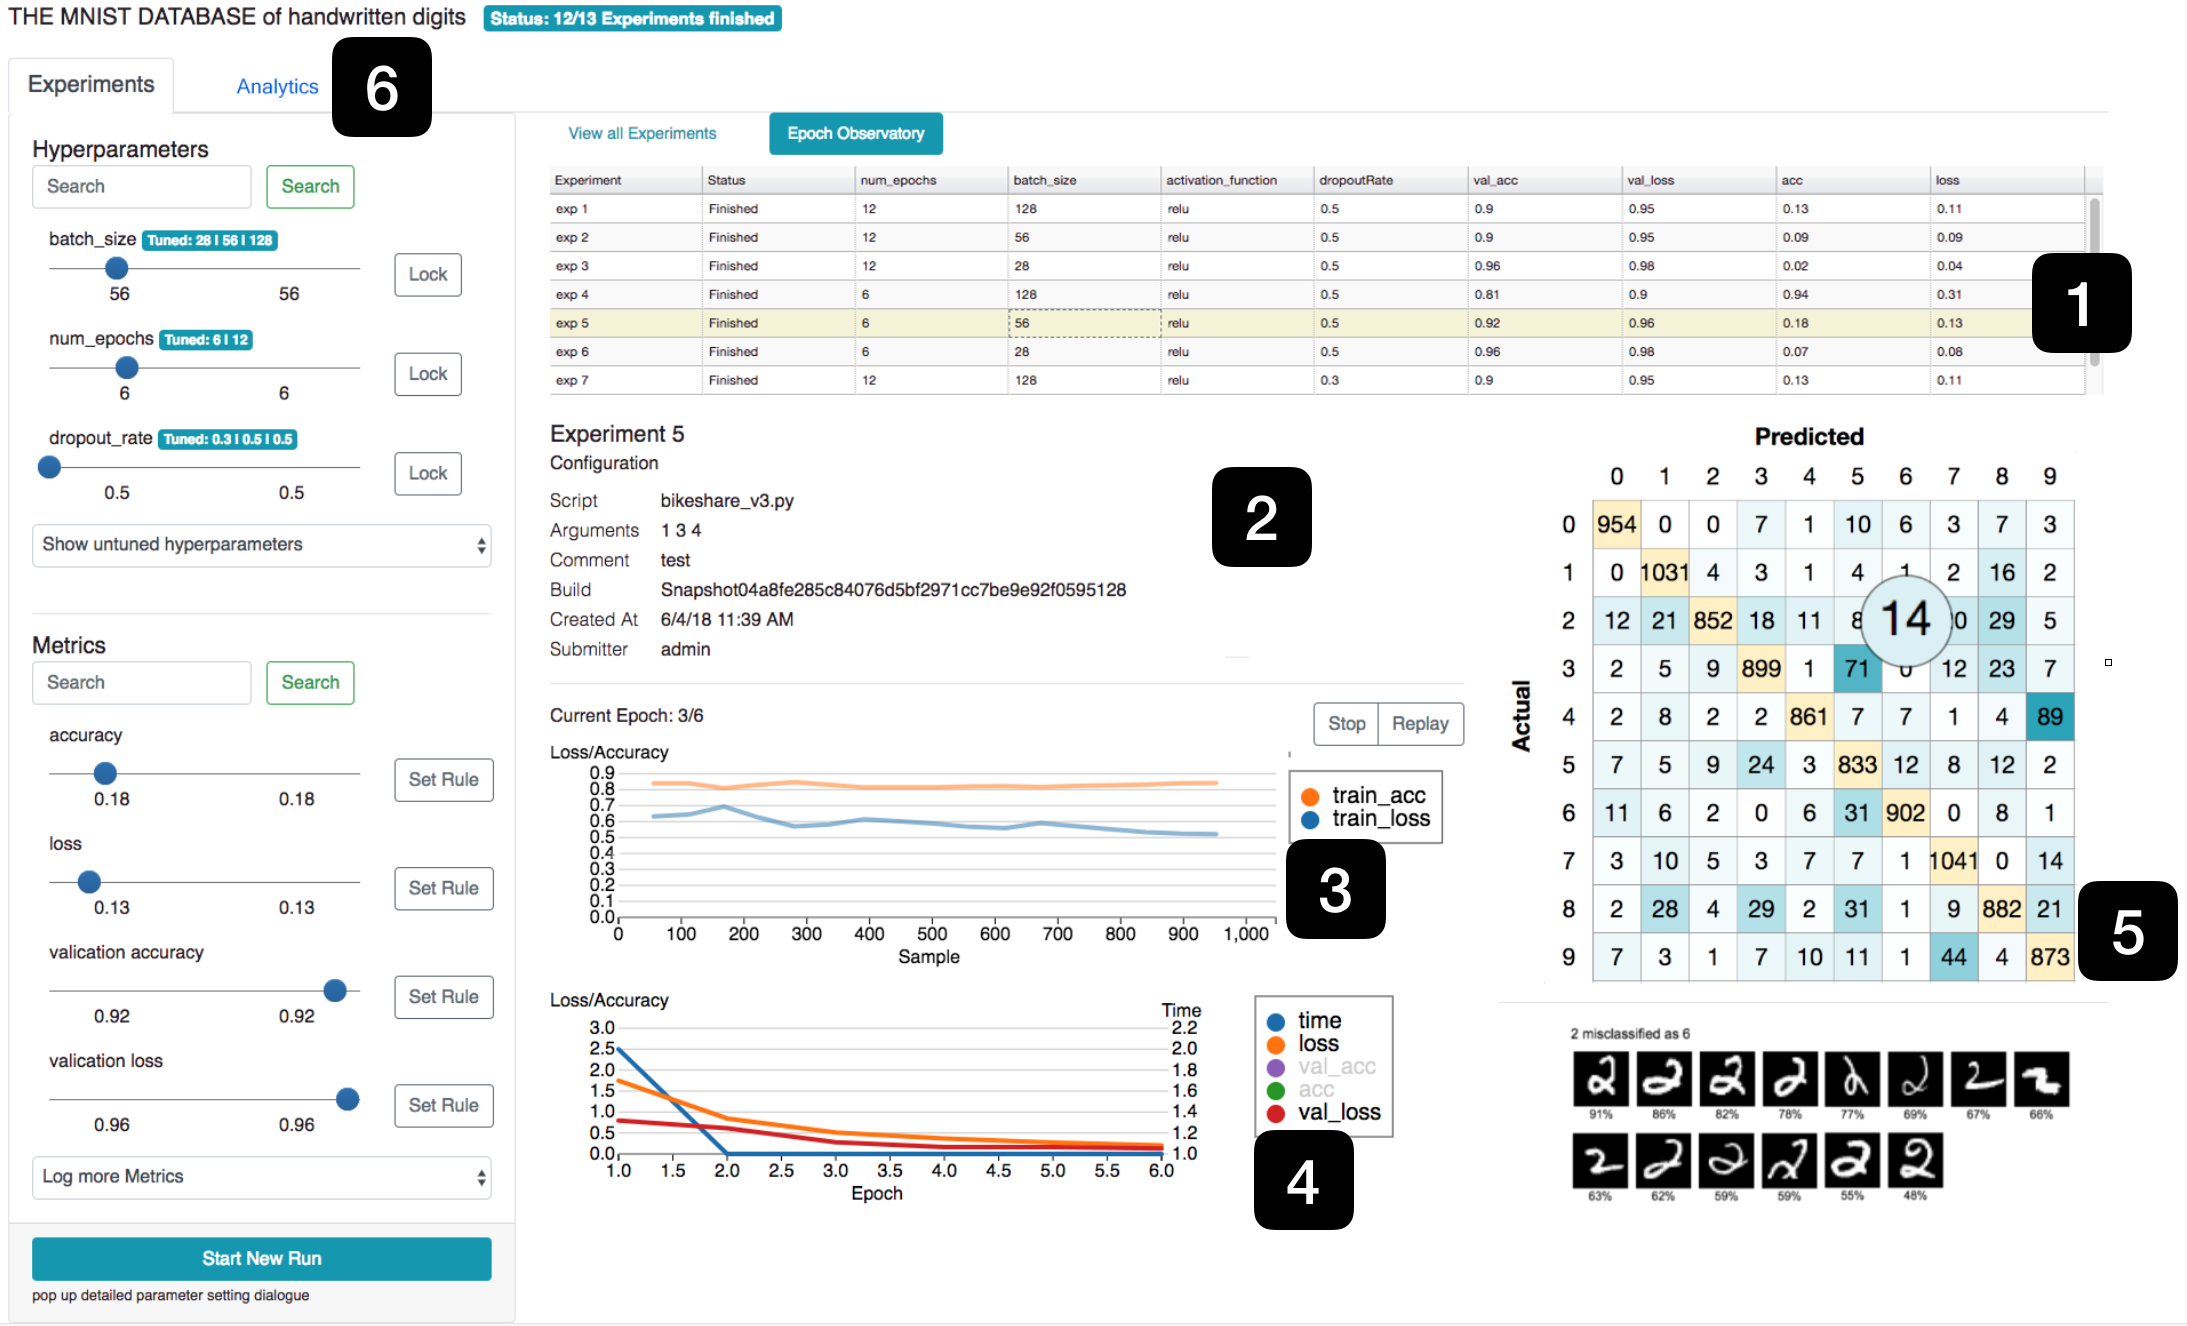
\includegraphics[width=\columnwidth]{pictures/epoch}
 \caption{Experiment dashboard for an individual experiment}
 \label{fig:local}
\end{figure}

\paragraph{Support to Decide the Next Batch of Experiments.} After examining the current experiment results in the global and local views back and forth, Sarah decided to run another batch of experiments, where she wants to set \textit{num\_epochs=12}, \textit{batch\_size=128}, \textit{dropout\_rate=0.7}, and experiment with a new hyperparameter: \textit{number of layers}. She clicks on "Start new run" on the bottom left and set a new grid of the hyperparameter values in a modal window with a similar interface to Figure \ref{fig:start}. As a result, as this new run is complete, the parameter panel in the run dashboard (see Figure \ref{fig:global} B.3 shown earlier) will now show four hyperparameters.

\subsection{Phase 2}
\paragraph{Project Dashboard.} Sarah has tuned the model across five batches of experiments and wants to save her progress so far as she feels satisfied by the results. While still in the Run Dashboard (where she analyzed her last run), she clicks on the "Analytics" tab (Figure \ref{fig:local} label 6) to analyze her progress across all runs in the Project Dashboard (Figure \ref{fig:allrun}) and then create a report. In this dashboard, she first scans the large table on the left with all the experiments she ran and with values of hyperparameter and performance metrics. Then she uses the line chart on the right to review how the performance metrics have improved run after run, historically (Figure \ref{fig:allrun}    upper right) in relation to the tuning of the hyperparameter values used (Figure \ref{fig:allrun} lower right). By brushing over the upper right chart, she selects all experiments from the first two runs and archives these in a group as the results were poor. Then she cleanses the set of experiments from the remaining three runs by interacting with the table on the left and using the checkboxes in the first column: she selects and archives the bad ones and stars a few good ones that she wants to discuss and annotate with her colleagues. Later on, after meeting her colleagues, she finally includes the best model in the report which she shares with the domain expert who requested the tuned model for a handwriting recognition application. 

\subsection{Prototype Status} The prototype implementation and evaluation are still in progress. Several components of the prototype, such as features of the project dashboard shown in Figure \ref{fig:allrun} (e.g., multi-selection, interactions over the charts on the right, and report sharing) are still under construction. The figures (\ref{fig:start}-\ref{fig:allrun}) and use cases in this section are intended to show how the final prototype will support the hyperparameter tuning process. Additional refinements to the prototype implementation are also expected after a final round of evaluation with the same practitioners.
\begin{figure}
 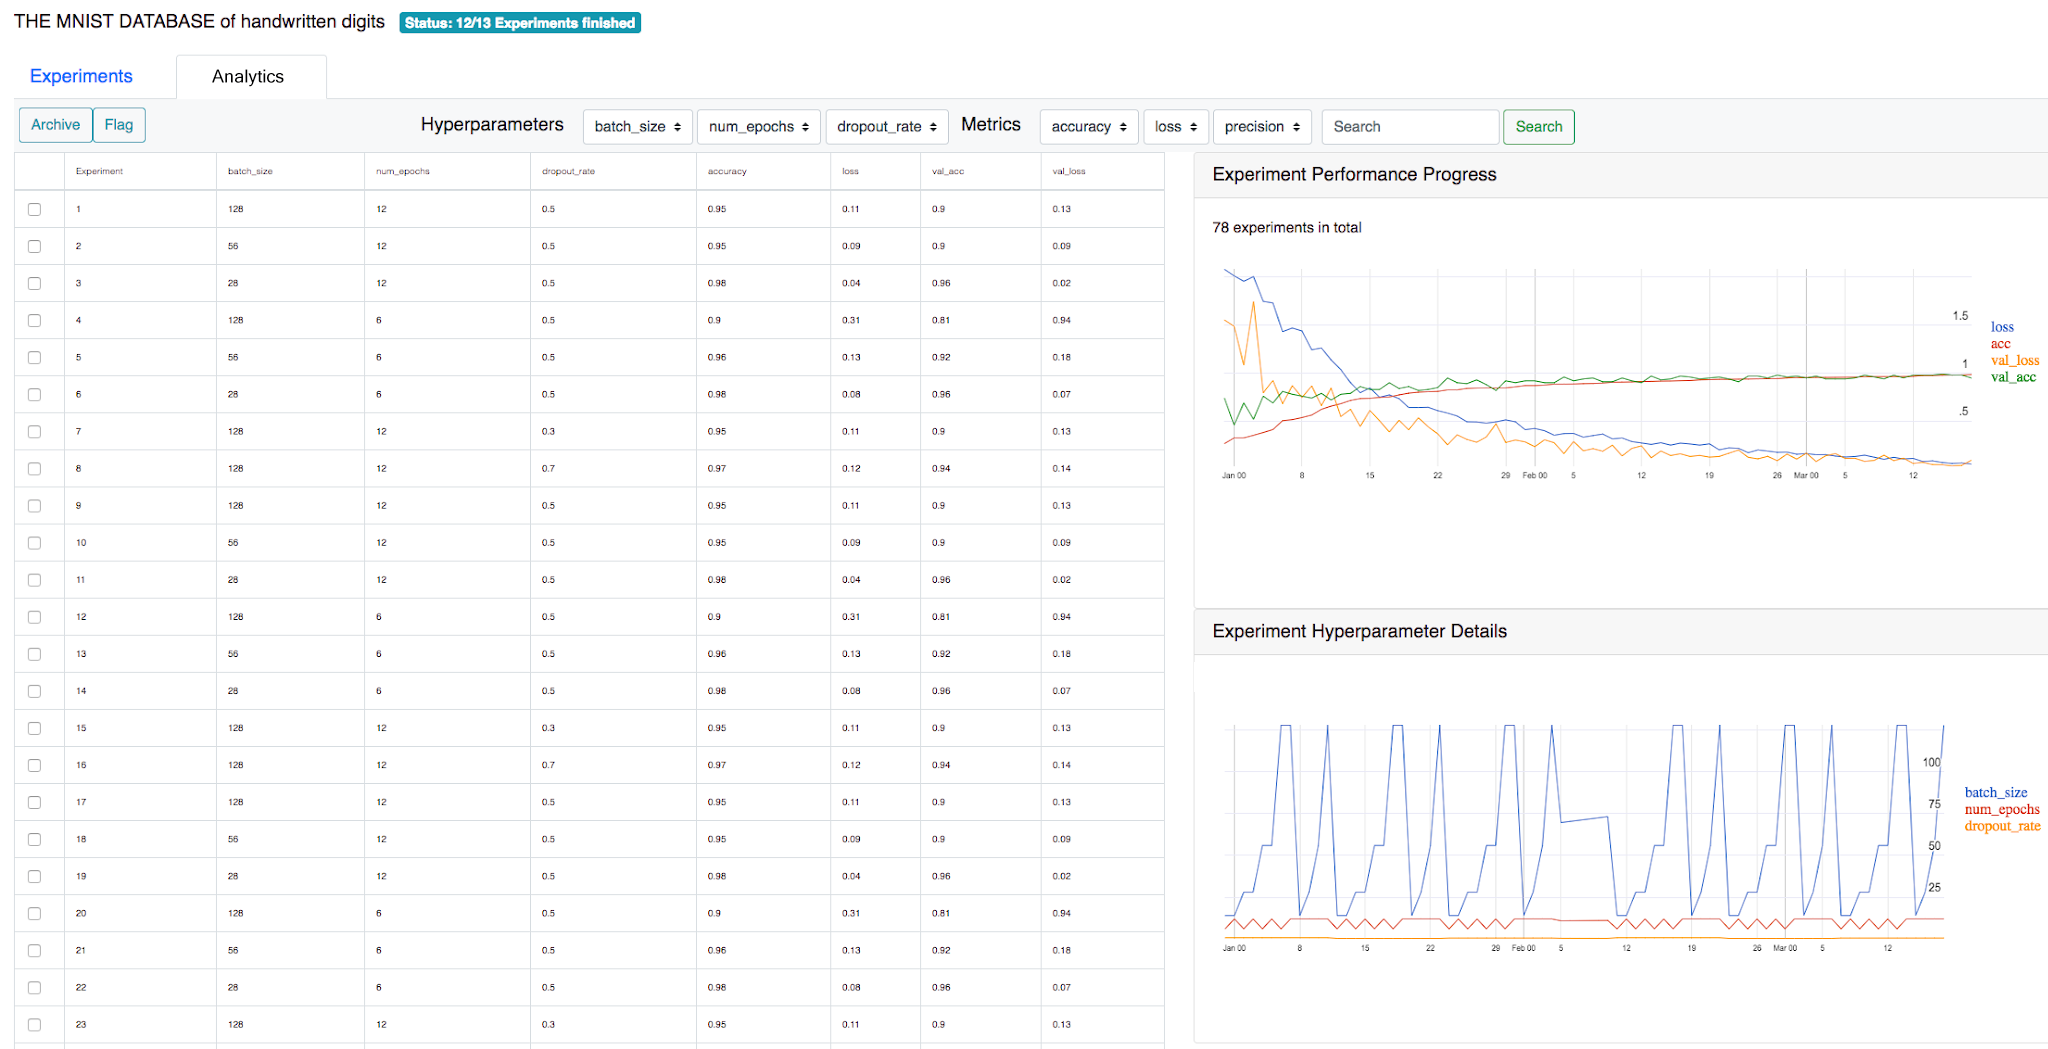
\includegraphics[width=\columnwidth]{pictures/allrun}
 \caption{Project Dashboard}
 \label{fig:allrun}
\end{figure}
% \begin{table}[tb]
%  \caption{VIS/VisWeek accepted/presented papers: 1990--2016.}
%  \label{tab:vis_papers}
%  \scriptsize%
%   \centering%
%  \begin{tabu}{%
%   r%
%   *{7}{c}%
%   *{2}{r}%
%   }
%  \toprule
%  year & \rotatebox{90}{Vis/SciVis} &  \rotatebox{90}{SciVis conf} &  \rotatebox{90}{InfoVis} &  \rotatebox{90}{VAST} &  \rotatebox{90}{VAST conf} &  \rotatebox{90}{TVCG @ VIS} &  \rotatebox{90}{CG\&A @ VIS} &  \rotatebox{90}{VIS/VisWeek} \rotatebox{90}{incl. TVCG/CG\&A}  &  \rotatebox{90}{VIS/VisWeek} \rotatebox{90}{w/o TVCG/CG\&A}  \\
%  \midrule
%   2016 & 30 &  & 37 & 33 & 15 & 23 & 10 & 148 & 115 \\
%  2015 & 33 & 9 & 38 & 33 & 14 & 17 & 15 & 159 & 127 \\
%  2014 & 34 &  & 45 & 33 & 21 & 20 &  & 153 & 133 \\
%  2013 & 31 &  & 38 & 32 &  & 20 &  & 121 & 101 \\
%  2012 & 42 &  & 44 & 30 &  & 23 &  & 139 & 116 \\
%  2011 & 49 &  & 44 & 26 &  & 20 &  & 139 & 119 \\
%  2010 & 48 &  & 35 & 26 &  &  &  & 109 & 109 \\
%  2009 & 54 &  & 37 & 26 &  &  &  & 117 & 117 \\
%  2008 & 50 &  & 28 & 21 &  &  &  & 99 & 99 \\
%  2007 & 56 &  & 27 & 24 &  &  &  & 107 & 107 \\
%  2006 & 63 &  & 24 & 26 &  &  &  & 113 & 113 \\
%  2005 & 88 &  & 31 &  &  &  &  & 119 & 119 \\
%  2004 & 70 &  & 27 &  &  &  &  & 97 & 97 \\
%  2003 & 74 &  & 29 &  &  &  &  & 103 & 103 \\
%  2002 & 78 &  & 23 &  &  &  &  & 101 & 101 \\
%  2001 & 74 &  & 22 &  &  &  &  & 96 & 96 \\
%  2000 & 73 &  & 20 &  &  &  &  & 93 & 93 \\
%  1999 & 69 &  & 19 &  &  &  &  & 88 & 88 \\
%  1998 & 72 &  & 18 &  &  &  &  & 90 & 90 \\
%  1997 & 72 &  & 16 &  &  &  &  & 88 & 88 \\
%  1996 & 65 &  & 12 &  &  &  &  & 77 & 77 \\
%  1995 & 56 &  & 18 &  &  &  &  & 74 & 74 \\
%  1994 & 53 &  &  &  &  &  &  & 53 & 53 \\
%  1993 & 55 &  &  &  &  &  &  & 55 & 55 \\
%  1992 & 53 &  &  &  &  &  &  & 53 & 53 \\
%  1991 & 50 &  &  &  &  &  &  & 50 & 50 \\
%  1990 & 53 &  &  &  &  &  &  & 53 & 53 \\
%  \midrule
%  \textbf{sum} & \textbf{1545} & \textbf{9} & \textbf{632} & \textbf{310} & \textbf{50} & \textbf{123} & \textbf{25} & \textbf{2694} & \textbf{2546} \\
%  \bottomrule
%  \end{tabu}%
% \end{table}

\subsection{Preliminary Evaluation}
We presented the workflow and the prototype to the same group of six data science practitioners as during the first phase. We used a similar method and each session lasted again an hour. During the session, we used screen sharing to first review the workflow (15 minutes) and then demonstrate each component of the interactive prototype (45 minutes). We used a semi-structured interview method with open-ended questions that requested feedback on the workflow and each prototype component. Each interviewee gave feedback and, when relevant, specified new requirements evoked by the prototype. We recorded and transcribed each session. The qualitative findings extracted by two co-authors from the transcripts are summarized below.

Overall, all interviewees validated that the workflow represents their current hyperparameter tuning process and captures the key sub-steps. The set of visual analytics capabilities supported in the prototype are useful and required. \textit{"I like the feature set, I can imagine myself using it. The handwritten notes stop making sense to me after a long time, and hard to understand for other people. The problem is: you just make up as you go along [reviewing the notes]. This structure will help formalize that." (Mk)}. In addition, the interviewees found the MNIST dataset and the CNN model used as content for the prototype implementation representative enough of hyperparameters and metrics used for real-world models. The prototype triggered further insights, where the interviewees gave suggestions of how the prototype could be connected or extended to help with work needed after the models are deployed in production (e.g., apply the model to new data). 

\paragraph{Run Dashboard.} 
The data science practitioners found the grid of hyperparameter-metric scatter plots and the brushing \& linking among all views particularly helpful as it fulfils a need not yet addressed by their tools. \textit{"It’s an inherently hard problem how you visualize multiple hyperparameters and performance [metrics]. But giving me the way to slice and dice it definitely helps."} About the line chart showing the performance metrics by experiment, this chart was initially designed as bar charts, then replaced by the current line chart to address scalability concerns by one of the interviewees who usually operate on hundreds of experiments. However, a second interviewee recommended reversing this design decision since connecting the performance with lines might be misleading: \textit{[The order of the experiments] does not follow a time series relationship ... there's no natural order to them, so I would argue this should be a bar graph, not a time series"}. Another recommended refinement of this chart is to find better solutions for performance metrics that have different scales and units: \textit{"I'm not a big fan of putting accuracy and loss in the same figure."} The visualization (e.g., axes) should interactively adjust based on the metrics selected and show multiple metrics in ways that help to compare a batch of experiments.

\paragraph{Experiment Dashboard.} 
Reviewing the epoch information of each experiment was a recurring practice among the interviewees. Moreover, they found the confusion matrix very helpful. This visualization is specific to the model and the data being used, thus it would be expensive to support across models. Our current prototype design partially addresses this problem by allowing extensions: for models that do not have an equivalent visualization, we leave it to the data science practitioner to plug in their own customized visualizations. However, the interviewees all suggested that it is still worth the efforts to pre-build some visualizations. \textit{I am willing to write extra lines of code to process the data so that it can be visualized this way. (Mk).} This suggests the need for pre-building commonly used visualizations as skeletons so that the users can populate with the training results of different models and/or datasets. 

\paragraph{Support to Decide the Next Batch of Experiments.} Keeping a panel of hyperparameters and performance metrics on the left in both run and experiment dashboards allows the user to keep track of their insights emerged from the analysis of the visualizations (Figure \ref{fig:global} B.3). All interviewees found the "lock" button in the parameter panel useful to record a promising range of values for a hyperparameter. In addition to this basic capability, it might help to have more advanced ways to capture insights during visual analysis. We explored with the interviewees the utility of defining and highlighting patterns in a visualization that may help locate the hyperparameter space worth exploring. For example, the user may build rules based on patterns in the form of threshold values for a metric (e.g., minimum accuracy required) or trend-line slope (e.g., positive or negative hyperparameter-metric relationship) over the hyperparameter-metric scatter plots. However, as the interviewees pointed out \textit{"the challenge is that the patterns are project-specific." (all)} and thus this type of advanced visual analytics support remains a challenge.

The evaluation of the parameter setting window (Figure \ref{fig:start}) suggested that a linear step size is usually not enough. Other common cases are logarithmic step sizes or other strategies. Some interviewees suggested that they would also like to manually type in the values in the argument line. Furthermore, they want to receive more feedback as they specify the parameters to be able to predict what would happen if they were to launch the batch of experiments. This refinement of the current design is motivated in particular by cases where the training might take days and require a large amount of computation. \textit{I would like to see if I do choose to use the linear step size, how many experiments and what will the combinations of hyperparameter values look like for each, just to make sure I didn't mess up with my math when setting step sizes. (Mk).} Another reason for showing this feedback is to allow the user to decide what to do with the combinations that have been already run. The interviewees pointed to good reasons why they would run the same hyperparameter value combination again: e.g. if the script or the data as changed in the meantime. That being said, the interviewees also wished they had recommendations on the best combinations to run: \textit{"Automatically display what happened when such combination was used would be the most useful thing to do." (Mk) "It could be helpful if the system can automatically recommend the ones with the highest potential success." (Mc)}. 

\paragraph{Project Dashboard.} 
The interviewees found it very useful to have a different level of visualizations that aggregates the model performance over time. These are \textit{"really valuable views because it's very easy to spin your wheels and make no progress without realizing it. "(Mk)}. Some also brought up the need to keep free notes. \textit{"Eight is a small number of experiments, and an interesting hyperparameter search is probably more than this. Then this starts to be challenging to find what you thought of yesterday." (Mc).} Archiving and flagging experiments are important, because over time as new data coming in, they want to flag what run to use in production. Such features help decide when to push a model to production and when to bring it out of production. Their common practice is to constantly update the test set to keep an eye on the model performance with the new data. There were also requirements on more visualizations, \textit{"I would also want to see the loss over epoch for multiple models[experiments] on the same graph. (Mc)"}.

\section{Discussion and Future Work}
% How our design can be generalized to other models
% How the prototype can be refined/enriched to satisfy the new requirements
% How our design fit into other research ecosystems (Connect to other research where they interpret model structures)
\subsection{Opportunity of learning from user interaction.}
% patterns, automatically highlight interesting experiments, recommending para and values, The importance of keep human in the loop of hyperparameter tuning.
An area of future work and discussion central to this workshop is about how visual analytics tools can allow data science practitioners to capture patterns on hyperparameter-metrics visualizations and use these patterns to guide the next round of hyperparameter tuning. In fact, identifying certain patterns is a central part of hyperparameter tuning. For instance, there is a known pattern that data science practitioners rely on to decide if the model is overfitting, which indicates that it's time to stop the training. The practice is to monitor both training loss and validation loss as a model is being trained. At the beginning, both the training loss and the validation loss values would decrease. Once the validation loss starts to increase, it means the model starts to overfit the training set of the data. This is a prevalently used pattern that can be predefined in visual analytics tools and be automatically flagged on occurrence in any project.
% This is a pattern that a visual analytics tool can allow the user to specify in a project (e.g., via an example) and then flag it as it re-occurs in other projects. 

However, most, if not all, of the other relevant patterns that a data science practitioners could use are project-specific, 
% specify on a visualization 
such as the slope of the training loss or the amount of noise (i.e., value fluctuations or variance) in the learning curve. 
% Yet what remains challenging is 
% The limited transferability of these patterns across projects. 
% Many of these patterns are specific to the project. 
Often there are no a priori rules, just comparisons afterwards. \textit{"I don't know what's good until I run what's bad. It's kind of important to understand what caused the noisy curve and how can I do to remedy noise in the future."} 
%Augmenting patterns and comparing the noisiest and least noisy experiments would be more helpful than rigidly setting a rule.
% 
% Another things is the slope of training loss, to see if it's sufficiently steep. This is problem specific so it's in comparison with other runs that will tell me that how good this run is and what is going on. Another thing is how noisy the loss curve is, and that will tell me whether I have too many or too little parameters or whether my learning rates are too high or too low, things like that. Or plateaus, there are all sorts of weird patterns that if you understand the model you can understand what is happening. The only universal thing is, you want the training loss to go down smoothly, the validation loss to go down smoothly, and then up. That's the ideal. Any other deviation from that is very project specific. The so-called rules are more like nuance.
% 
% It's worth noting, however, that it's because of this very lack of a priori rules 
The limited transferability of these patterns across projects (and because of external factors such as performance expectations and resources not specified in the tool) makes it essential to keep human in the loop and learn about ad-hoc user interaction to provide project-specific support.
% to efficiently identify the sweet spot of hyperparameters. 
This point was stated emphatically by one of the interviewees (Mc): \textit{"hyperparameter tuning is a special part of machine learning, ... an art that doesn't have many libraries or rules of thumb. There are no rules to indicate when to apply what. It's all about trial and errors but because of that it requires experience to know which trials you will never even start doing."} 
 
% One repetitive but ad hoc process is sometimes the data science practitioners might want to abandon experiments before the training completes because they could cause quite expensive computations, taking several days. For example, the loss function is the quantity to minimize; the value will first go down during the experiment, and then at some point, it might start going up, at which point the user might want to stop the experiment. It is not because the results are getting worse since it's always possible to recover the situation when it's at its best, but clearly, it is wasting CPU cycles now because the performance of the model is degrading and it's unlikely to improve. 
% % that the data science practitioners need to filter out bad experiments and highlight interesting ones. Sometimes you
% The other thing is, when training hundreds of experiments if the performance metrics start to converge after ten, and it doesn't get any better or worse, it would save time and money to stop at 12 or 15, rather than going all the way. It can be quite heuristic and project-dependent. Customized learning of user interaction in each project would be a valuable direction to investigate in future work.



\subsection{Modularized workflow and automation.}
% plug in random search
Another area of future work and discussion is about alternative strategies to search the parameter space and how they could be combined modularly depending on the project needs. The approach we advocated in this paper is an interactive form of grid search where the human steers the search process based on insights s/he collects at each iteration until s/he settles on some of the hyperparameter values. 
% The prototype get the data science practitioners in writing complicated search scripts to interactively analyzing the search progress. However, this approach can be integrated with automation. 
The modularization of the workflow we proposed would allow plugging in automated search technology. For example, an automated random search can be initiated by randomly sampling the candidate values from a user-specified range. Then after the experiments are completed by this automatic module, the results can be used to fit in certain statistical models, depending on the optimization algorithm.

% \subsection{Modularized workflow and automation.} OLD version
% % plug in random search
% It's convenient that the interface allows the user to select which hyperparameter to tune next, as s/he settles on some of the hyperparameter values (either found the sweet spot or figured it has less impact/importance). The prototype gets the data science practitioners from writing complicated search scripts to interactively analyzing the search progress. It is a relatively naive strategy to interactively go through small search grids and expand to the previously untuned hyperparameters across the entire search space. However, the modularization can enable future extensions to plug in more advanced search technology. For example, instead of setting the hyperparameter candidate values by interval and steps, a random search strategy can be supported by randomly sampling the candidate values from a user-specified range. After the experiments are completed, the results can be used to fit in certain statistical models of the user's choice.
% \paragraph{Save to by automating repeated practices.} Automatically generate the commonly used visualizations (like the pairwise comparison scatter plots) visual would save time. Currently, this steps is \textit{“really time-consuming” (Jm)}. It’s important to design the prototype to help with the things that are repeated over and over again, where we can save the most amount of the time. 

 

\acknowledgments{\note{if specified like this the section will be committed in review mode}

The authors wish to thank the data science practitioners for their time and active participation and our collaborators in the UX and CDSW teams at Cloudera for their support.}

%\bibliographystyle{abbrv}
\bibliographystyle{abbrv-doi}
%\bibliographystyle{abbrv-doi-narrow}
%\bibliographystyle{abbrv-doi-hyperref}
%\bibliographystyle{abbrv-doi-hyperref-narrow}

\bibliography{Mendeley_Cloudera_Data_Science_Workbench}
\end{document}




\subsection{Balancing generalizability and customized analysis.}
We demonstrate the prototype with an example project that uses CNN model to classify MNIST dataset. Most of the visualizations only concern the number and data types of the hyperparameters and performance metrics, which do not make assumptions about the type of the model. The confusion matrix we demonstrated in the individual experiment dashboard is meant to be customized by the user for more ad-hoc analysis during the tuning process.
\paragraph{Feasibility.} However, we did make an assumption that all the hyperparameter and performance metrics are tracked and the values are available for visualization. One of the interviewees raised the concern regarding how the interface talks to the scripts. One possibility is to eliminate the code for hyperparameter search and launch the script as many times as the number of combination of hyperparameter values. This will make it much easier to make sense of different experiments as well. And the person who writes the scripts does not have to update the code every time there is a need to start a new hyperparameters tuning process.

